%%
% The BIThesis Template for Bachelor Graduation Thesis
%
% 北京理工大学毕业设计(论文) —— 使用 XeLaTeX 编译
%
% Copyright 2021 BITNP
%
% This work may be distributed and/or modified under the
% conditions of the LaTeX Project Public License, either version 1.3
% of this license or (at your option) any later version.
% The latest version of this license is in
%   http://www.latex-project.org/lppl.txt
% and version 1.3 or later is part of all distributions of LaTeX
% version 2005/12/01 or later.
%
% This work has the LPPL maintenance status `maintained'.
%
% The Current Maintainer of this work is Feng Kaiyu.
%
% Compile with: xelatex -> biber -> xelatex -> xelatex

% 章节支持、单面打印:ctexbook
\documentclass[bachelor,footskip=24pt]{bitbook}
% 如果想要修改样式,但无法找到样式在哪里定义:请参考 https://bithesis.bitnp.net/Guide/4-Others/Troubleshooting.html#%E6%83%B3%E8%A6%81%E4%BF%AE%E6%94%B9%E9%83%A8%E5%88%86%E6%A0%B7%E5%BC%8F-%E4%BD%86%E6%98%AF%E6%89%BE%E4%B8%8D%E5%88%B0%E6%A0%B7%E5%BC%8F%E5%9C%A8%E5%93%AA%E9%87%8C%E5%AE%9A%E4%B9%89

% 另一个临时的“修改页眉文字”的解决方法(非常不优雅,只作为临时措施)。
% 请注释掉以下 20 行内容使用。
% % 从原有主题继承自定义主题
% \fancypagestyle{BIThesisCustom}[BIThesis]{
%   % 定义页眉、页码
%   \fancyhead[C]{\zihao{4}\ziju{0.08}\songti{ }}
% }
% % 设置章节格式
% \ctexset{chapter={
%     pagestyle = BIThesisCustom,
%   }
% }
% % 前置页面(原创性声明、中英文摘要、目录等)
% \renewcommand{\frontmatter}{
%   \pagenumbering{Roman}
%   \pagestyle{BIThesisCustom}
% }
% % 正文页面
% \renewcommand{\mainmatter}{
%   \pagenumbering{arabic}
%   \pagestyle{BIThesisCustom}
% }
% ------------------------------------------------------------------

% 使用 listings 宏包进行代码块使用,并使用了预定义的样式,
% 你也可以选用自己的喜欢的其他宏包,如 minted;
% 然而由于 minted 依赖 Python 的 Pygments 库作为外部依赖,因此出于模板的建议性考虑,我们没有提供 minted 进行代码块书写的示例。
% 但是,我们仍旧非常建议你使用 minted。
\usepackage{listings}
\usepackage[ruled]{algorithm2e}
\usepackage{subfigure}
\usepackage{url}

% 参考文献引用文件位于 misc/ref.bib
\addbibresource{misc/ref.bib}

% 在这里填写你的论文中英文题目
\newcommand{\thesisTitle}{基于深度强化学习的自动驾驶避障技术研究}
\newcommand{\thesisTitleEN}{Research on Automatic Driving Obstacle Avoidance Based on Deep Reinforcement Learning}

% 在这里填写你的相关信息
\newcommand{\deptName}{自动化学院}
\newcommand{\majorName}{自动化}
\newcommand{\yourName}{黄宸睿}
\newcommand{\yourStudentID}{1120181506}
\newcommand{\mentorName}{宋春雷}
% 如果你的毕设为校外毕设,请将下面这一行语句解除注释(删除第一个百分号字符)并在第二组花括号中填写你的校外毕设导师名字
% \newcommand{\externalMentorName}{左偏树}

% 文档开始
\begin{document}

% 标题页面:如无特殊需要,本部分无需改动
%%
% The BIThesis Template for Bachelor Graduation Thesis
%
% 北京理工大学毕业设计(论文)封面页 —— 使用 XeLaTeX 编译
%
% Copyright 2020-2021 BITNP
%
% This work may be distributed and/or modified under the
% conditions of the LaTeX Project Public License, either version 1.3
% of this license or (at your option) any later version.
% The latest version of this license is in
%   http://www.latex-project.org/lppl.txt
% and version 1.3 or later is part of all distributions of LaTeX
% version 2005/12/01 or later.
%
% This work has the LPPL maintenance status `maintained'.
%
% The Current Maintainer of this work is Feng Kaiyu.
%
% 封面
%
% 如无特殊需要,本页面无需更改

% Underline new command for student information
% Usage: \dunderline[<offset>]{<line_thickness>}
\newcommand\dunderline[3][-1pt]{{%
  \setbox0=\hbox{#3}
  \ooalign{\copy0\cr\rule[\dimexpr#1-#2\relax]{\wd0}{#2}}}}

% Cover Page
\begin{titlepage}
  \makeatletter
  \@ifundefined{externalMentorName}{
    % 校内毕设封面顶部间距
    \vspace*{19mm}
  }{
    % 校外毕设封面顶部间距
    \vspace*{13mm}
  }
  \centering

  
\includegraphics[width=9.87cm]{images/header.png}

  \vspace*{-3mm}

  \zihao{-0}\textbf{\ziju{0.12}\songti{本科生毕业设计(论文)}}

  \vspace{16mm}

  \zihao{2}\textbf{\xihei\thesisTitle}

  \vspace{3mm}

  \begin{spacing}{1.2}
    \zihao{3}\selectfont{\textbf{\thesisTitleEN}}
  \end{spacing}

  \vspace{15mm}

  \flushleft

  \makeatletter
  \@ifundefined{externalMentorName}{
    % 生成校内毕设封面字段
    \makeatother
    \begin{spacing}{1.8}
      \hspace{27mm}\songti\zihao{3}\selectfont{学\hspace{11mm}院:\dunderline[-10pt]{1pt}{\makebox[78mm][c]{\deptName}}}

      \hspace{27mm}\songti\zihao{3}\selectfont{专\hspace{11mm}业:\dunderline[-10pt]{1pt}{\makebox[78mm][c]{\majorName}}}

      \hspace{27mm}\songti\zihao{3}\selectfont{学生姓名:\dunderline[-10pt]{1pt}{\makebox[78mm][c]{\yourName}}}

      \hspace{27mm}\songti\zihao{3}\selectfont{学\hspace{11mm}号:\dunderline[-10pt]{1pt}{\makebox[78mm][c]{\yourStudentID}}}

      \hspace{27mm}\songti\zihao{3}\selectfont{指导教师:\dunderline[-10pt]{1pt}{\makebox[78mm][c]{\mentorName}}}
    \end{spacing}
  }{
    % 生成校外毕设封面字段
    \makeatother
    \begin{spacing}{1.8}
      \hspace{19.4mm}\songti\zihao{3}\selectfont{学\hspace{19.6mm}院\hspace{3mm}:\dunderline[-10pt]{1pt}{\makebox[77.4mm][c]{\deptName}}}

      \hspace{19.4mm}\songti\zihao{3}\selectfont{专\hspace{19.6mm}业\hspace{3mm}:\dunderline[-10pt]{1pt}{\makebox[77.4mm][c]{\majorName}}}

      \hspace{19.4mm}\songti\zihao{3}\selectfont{学\hspace{2.8mm}生\hspace{2.8mm}姓\hspace{2.8mm}名\hspace{3mm}:\dunderline[-10pt]{1pt}{\makebox[77.4mm][c]{\yourName}}}

      \hspace{19.4mm}\songti\zihao{3}\selectfont{学\hspace{19.6mm}号\hspace{3mm}:\dunderline[-10pt]{1pt}{\makebox[77.4mm][c]{\yourStudentID}}}

      \hspace{19.4mm}\songti\zihao{3}\selectfont{指\hspace{2.8mm}导\hspace{2.8mm}教\hspace{2.8mm}师\hspace{3mm}:\dunderline[-10pt]{1pt}{\makebox[77.4mm][c]{\mentorName}}}

      \hspace{19.4mm}\songti\zihao{3}\selectfont{校外指导教师:\dunderline[-10pt]{1pt}{\makebox[77.4mm][c]{\externalMentorName}}}
    \end{spacing}
  }

  \vspace*{\fill}
  \centering
  \zihao{3}\ziju{0.5}\songti{\today}
\end{titlepage}


% 前置页面定义
\frontmatter
% 原创性声明:如无特殊需要,本部分无需改动
% 更改为 PDF 页面插入,如需要添加内容,可考虑先用 Word 制作再覆盖 misc/1_originality.pdf

\includepdf{misc/1_originality.pdf}
\newpage
%%%
% The BIThesis Template for Bachelor Graduation Thesis
%
% 北京理工大学毕业设计(论文)原创性声明页 —— 使用 XeLaTeX 编译
%
% Copyright 2020-2021 BITNP
%
% This work may be distributed and/or modified under the
% conditions of the LaTeX Project Public License, either version 1.3
% of this license or (at your option) any later version.
% The latest version of this license is in
%   http://www.latex-project.org/lppl.txt
% and version 1.3 or later is part of all distributions of LaTeX
% version 2005/12/01 or later.
%
% This work has the LPPL maintenance status `maintained'.
%
% The Current Maintainer of this work is Feng Kaiyu.
%
% 如无特殊需要,本页面无需更改

% 原创性声明页无页码页面格式
\fancypagestyle{originality}{
  % 页眉高度
  \setlength{\headheight}{20pt}

  % 页眉和页脚(页码)的格式设定
  \fancyhf{}
  \fancyhead[C]{\zihao{4}\ziju{0.08}\songti{北京理工大学本科生毕业设计(论文)}}

  % 页眉分割线稍微粗一些
  \renewcommand{\headrulewidth}{0.6pt}
}

\pagestyle{originality}
\topskip=0pt

% 圆形数字编号定义
\newcommand{\circled}[2][]{\tikz[baseline=(char.base)]
  {\node[shape = circle, draw, inner sep = 1pt]
  (char) {\phantom{\ifblank{#1}{#2}{#1}}};
  \node at (char.center) {\makebox[0pt][c]{#2}};}}
\robustify{\circled}

% 设置行间距
\setlength{\parskip}{0.4em}
\renewcommand{\baselinestretch}{1.41}

% 顶部空白
\vspace*{-6mm}

% 原创性声明部分
\begin{center}
  \heiti\zihao{2}\textbf{原创性声明}
\end{center}

% 本部分字号为小三
\zihao{-3}

本人郑重声明:所呈交的毕业设计(论文),是本人在指导老师的指导下独立进行研究所取得的成果。除文中已经注明引用的内容外,本文不包含任何其他个人或集体已经发表或撰写过的研究成果。对本文的研究做出重要贡献的个人和集体,均已在文中以明确方式标明。

特此申明。

\vspace{13mm}

\begin{flushright}
  本人签名:\hspace{40mm}日\hspace{2.5mm}期:\hspace{13mm}年\hspace{8mm}月\hspace{8mm}日
\end{flushright}

\vspace{17mm}

% 使用授权声明部分
\begin{center}
  \heiti\zihao{2}\textbf{关于使用授权的声明}
\end{center}

本人完全了解北京理工大学有关保管、使用毕业设计(论文)的规定,其中包括:\circled{1}学校有权保管、并向有关部门送交本毕业设计(论文)的原件与复印件;\circled{2}学校可以采用影印、缩印或其它复制手段复制并保存本毕业设计(论文);\circled{3}学校可允许本毕业设计(论文)被查阅或借阅;\circled{4}学校可以学术交流为目的,复制赠送和交换本毕业设计(论文);\circled{5}学校可以公布本毕业设计(论文)的全部或部分内容。

\vspace*{1mm}

\begin{flushright}
  \begin{spacing}{1.65}
    \zihao{-3}
    本人签名:\hspace{40mm}日\hspace{2.5mm}期:\hspace{13mm}年\hspace{8mm}月\hspace{8mm}日\\
    指导老师签名:\hspace{40mm}日\hspace{2.5mm}期:\hspace{13mm}年\hspace{8mm}月\hspace{8mm}日
  \end{spacing}
\end{flushright}

\newpage

% 摘要:在摘要相应的 TeX 文件处进行摘要部分的撰写
%%
% The BIThesis Template for Bachelor Graduation Thesis
%
% 北京理工大学毕业设计(论文)中英文摘要 —— 使用 XeLaTeX 编译
%
% Copyright 2020-2021 BITNP
%
% This work may be distributed and/or modified under the
% conditions of the LaTeX Project Public License, either version 1.3
% of this license or (at your option) any later version.
% The latest version of this license is in
%   http://www.latex-project.org/lppl.txt
% and version 1.3 or later is part of all distributions of LaTeX
% version 2005/12/01 or later.
%
% This work has the LPPL maintenance status `maintained'.
%
% The Current Maintainer of this work is Feng Kaiyu.

% 中英文摘要章节
\zihao{-4}
\vspace*{-11mm}

\begin{center}
  \heiti\zihao{-2}\textbf{\thesisTitle}
\end{center}

\vspace*{2mm}

{\let\clearpage\relax \chapter*{\textmd{摘~~~~要}}}
\addcontentsline{toc}{chapter}{摘~~~~要}
\setcounter{page}{1}

\vspace*{1mm}

\setstretch{1.53}
\setlength{\parskip}{0em}

% 中文摘要正文从这里开始
自动驾驶系统保证了快捷、安全、高效的驾驶体验,实现自动驾驶避障需要自动驾驶决策和控制系统的紧密配合。强化学习通过不断探索环境,自主学习复杂的控制模型,深度学习与强化学习相结合形成的深度强化学习方法可实现端到端的决策与控制,逐渐成为自动驾驶领域的研究热点。本文以实现端到端的自动驾驶决策器和控制器作为研究目标,围绕两种不同复杂度的仿真环境,针对DQN及其改进算法搭建神经网络模型开展了相关技术研究,主要研究内容如下:

(1)针对强化学习的相关算法选择,第2章通过对强化学习算法原理的分析,引出了适用于无模型的 Q-learning 算法和 DQN 算法,针对于DQN算法的不足和缺陷,介绍了Double DQN算法和Dueling DQN算法的原理,并对DQN及其改进算法的适用场景进行了分析。

(2)针对自动驾驶避障算法,第3章完成了自动驾驶决策器与控制器的算法设计。通过对两种仿真环境(Highway-Env、Metadrive)状态值、动作值与奖励函数的对比与分析,设计了DQN及其改进算法的网络结构及超参数,对自动驾驶决策器与控制器的学习过程进行分析,使其完成自动驾驶决策和控制两方面的任务要求。

(3)针对实验验证,第4章进行了两种仿真环境中决策器与控制器的实验,验证了提出的自动驾驶避障算法的可行性和有效性,并对具体的实验内容进行了设计,对最终的实验结果进行了详细的分析与改进。

实验结果表明,本文设计实现的基于DQN及其改进算法的自动驾驶决策器和控制器均满足实验要求,达到了预期的控制效果,能够有效提高自动驾驶车辆在决策和控制中的鲁棒性。对于较为简单的网络结构,DQN特别是Double DQN算法由于其改进的动作选择和评估方法,能够获得更加稳定有效的行为策略。本文的成果为自动驾驶决策器和控制器的研究提供了借鉴和参考,也为复杂动力学模型问题的解决提供了新的思路和方法。

\vspace{4ex}\noindent\textbf{\heiti 关键词:自动驾驶避障;自动驾驶决策;控制器设计;DQN网络;深度强化学习;端到端驾驶}
\newpage

% 英文摘要章节
\vspace*{-2mm}

\begin{spacing}{0.95}
  \centering
  \heiti\zihao{3}\textbf{\thesisTitleEN}
\end{spacing}

\vspace*{17mm}

{\let\clearpage\relax \chapter*{
  \zihao{-3}\textmd{Abstract}\vskip -3bp}}
\addcontentsline{toc}{chapter}{Abstract}
\setcounter{page}{2}

\setstretch{1.53}
\setlength{\parskip}{0em}

% 英文摘要正文从这里开始
The Automatic Driving System ensures a fast, safe and efficient driving experience. The implementation of Automatic Driving Obstacle Avoidance requires the cooperation of the decision-making and control system of Automatic Driving. Reinforcement Learning learns complex control models autonomously by exploring the environment continuously. The Deep Reinforcement Learning method, formed by the combination of Deep Learning and Reinforcement Learning,  can realize end-to-end decision-making and control, and has gradually become a research hotspot in the field of Autonomous Driving. This work aims to implement the end-to-end Autonomous Driving decision maker and controller. Focusing on two simulation environments with different complexity, a neural network model is built for DQN and its improved algorithms. The performance is verified. The main research contents are as follows:

(1) For the selection of relevant algorithms for Reinforcement Learning, the second chapter analyses the principle of Reinforcement Learning algorithm, introduces the Q-learning algorithm and DQN algorithm suitable for model-free. In view of the shortcomings and defects of DQN algorithm, the principles of Double DQN algorithm and Dueling DQN algorithm are introduced, and the applicable scenarios of DQN and its improved algorithm are analyzed.

(2) For the Automatic Driving Obstacle Avoidance algorithm, the third chapter completes the algorithm design of the Automatic Driving decision maker and controller. Through the comparison and analysis of the state value, action value and reward function of the two simulation environments (Highway-Env, Metadrive), the network structure and hyperparameters of DQN and its improved algorithm are designed. 

(3) For the experimental verification, the fourth chapter conducts experiments on the decision maker and controller in two simulation environments, verifies the feasibility and effectiveness of the proposed Automatic Driving Obstacle Avoidance algorithm, the final experimental results are analyzed and improved in detail.

The experimental results show that the Autonomous Driving decision maker and controller based on DQN and its improved algorithms designed and implemented in this work meet the experimental requirements, achieve the expected control effect, and can effectively improve the robustness of autonomous driving vehicles in decision-making and control. For simpler network structures, DQN, especially the Double DQN algorithm, can obtain more stable and effective behavior strategies due to its improved action selection and evaluation methods. The results of this work provide reference for the research of Automatic Driving decision maker and controller, and also provide new ideas and methods for solving complex dynamic model problems.

\vspace{3ex}\noindent\textbf{Key Words: Automatic Driving Obstacle Avoidance; Automatic Driving Decision-Making; Controller Design; DQN Network; Reinforcement Learning; End-to-end Driving}
\newpage

% 目录:如无特殊需要,本部分无需改动
%%
% The BIThesis Template for Bachelor Graduation Thesis
%
% 北京理工大学毕业设计(论文)目录 —— 使用 XeLaTeX 编译
%
% Copyright 2020-2021 BITNP
%
% This work may be distributed and/or modified under the
% conditions of the LaTeX Project Public License, either version 1.3
% of this license or (at your option) any later version.
% The latest version of this license is in
%   http://www.latex-project.org/lppl.txt
% and version 1.3 or later is part of all distributions of LaTeX
% version 2005/12/01 or later.
%
% This work has the LPPL maintenance status `maintained'.
%
% The Current Maintainer of this work is Feng Kaiyu.
%
% 如无特殊需要,本页面无需更改

% 目录开始

% 调整目录行间距
\renewcommand{\baselinestretch}{1.35}
% 目录
\tableofcontents
\newpage


% 正文开始
\mainmatter
% 正文 22 磅的行距
\setlength{\parskip}{0em}
\renewcommand{\baselinestretch}{1.53}
% 修复脚注出现跨页的问题
\interfootnotelinepenalty=10000

% 第一章
%%
% The BIThesis Template for Bachelor Graduation Thesis
%
% 北京理工大学毕业设计(论文)第一章节 —— 使用 XeLaTeX 编译
%
% Copyright 2020-2021 BITNP
%
% This work may be distributed and/or modified under the
% conditions of the LaTeX Project Public License, either version 1.3
% of this license or (at your option) any later version.
% The latest version of this license is in
%   http://www.latex-project.org/lppl.txt
% and version 1.3 or later is part of all distributions of LaTeX
% version 2005/12/01 or later.
%
% This work has the LPPL maintenance status `maintained'.
%
% The Current Maintainer of this work is Huang Chenrui.
%
% 第一章节 2022/05/10

\chapter{绪论} % 引出要研究的是DQN,这是重点

\section{研究背景与意义}\label{1.1研究背景与意义} % 主要讲深度强化学习好,所以我们要研究它。

自动驾驶系统的决策模块需要先进的决策算法保证安全性、智能性、有效性。目前传统算法的解决思路是以价格昂贵的激光雷达作为主要传感器,依靠人工设计的算法从复杂环境中提取关键信息, 根据这些信息进行决策和判断。该算法缺乏一定的泛化能力,不具备应有的智能性和通用性。深度强化学习的出现有效地改善了传统算法泛化性不足的问题, 这给智能驾驶领域带来新的思路。

强化学习(Reinforcement Learning, RL)通过与环境交互,学习状态到行为的映射关系。如图\ref{强化学习原理}所示,在一个离散时间序列$t=0,1,2,… $中,智能体需要完成某项任务。在每一个时间$t$,智能体都能从环境中接受一个状态$S_t$,并通过动作$a_t$与环境继续交互,环境会产生新的状态$S_{t+1}$,同时给出一个立即回报$r_{t+1}$。如此循环下去,智能体与环境不断地交互,从而产生更多数据(状态和回报),并利用新的数据进一步改善自身的行为。

\begin{figure}[htbp]
  \vspace{13pt} % 调整图片与上文的垂直距离
  \centering
  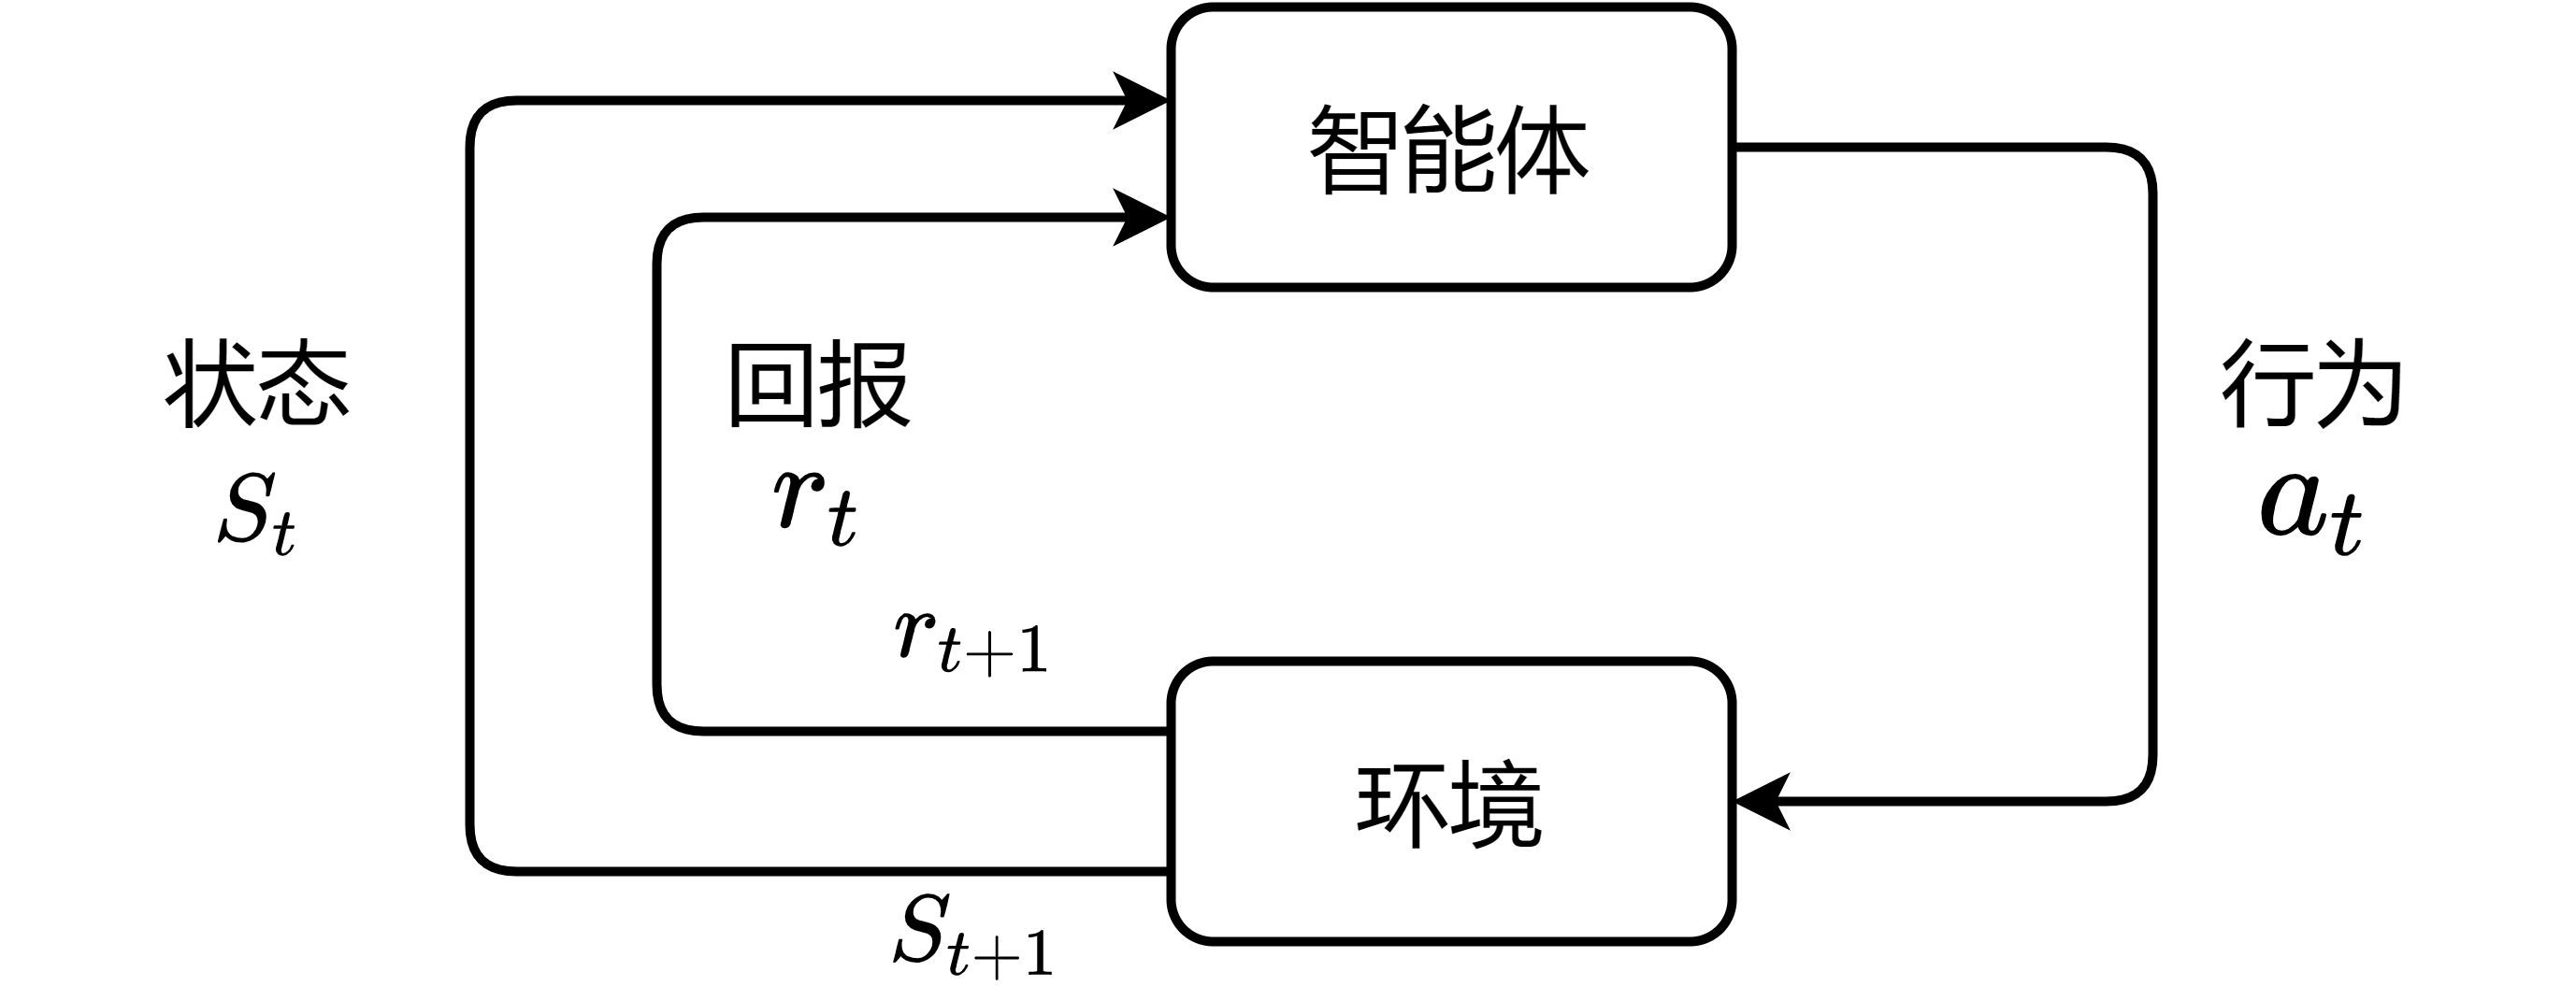
\includegraphics[width=0.73\textwidth]{images/chapter1/RL_structure.png}
  \caption{强化学习原理}\label{强化学习原理} % label 用来在文中索引
\end{figure}

目前,强化学习在策略选择的理论和算法方面已经取得了很大的进步,然而直接从高维感知输入(如图像、语音等)中提取特征,学习最优策略,对强化学习来说依然是一个挑战。

深度强化学习(Deep Reinforcement Learning, DRL)结合了深度神经网络和强化学习的优势, 可以用于解决智能体在复杂高维状态空间中的感知决策问题\cite{唐振韬2017深度强化学习进展}\cite{2017Deep}。2016年,基于深度强化学习和蒙特卡洛树搜索的AlphaGo击败了人类顶尖职业棋手,引起了全世界的关注\cite{2017Review}。 2017年, DeepMind在《Nature》上公布了最新版AlphaGo论文, 介绍了更强的围棋人工智能: AlphaGo Zero。它不需要人类专家知识, 只使用纯粹的深度强化学习技术和蒙特卡罗树搜索, 经过3天自我对弈就以100比0击败了上一版本的AlphaGo。AlphaGo Zero证明了深度强化学习的强大能力, 也必将推动以深度强化学习为代表的人工智能领域的进一步发展。基于深度强化学习在棋局与游戏上的成功,最近的研究大多注重于深度强化学习在各个领域中的扩展与应用。

综上所述,深度强化学习方法与深度神经网络强大的特征提取能力相结合,可以实现端到端的控制与决策,具有较强的通用性。通过网络自主学习的方式,减少了对系统动力学建模与数学解析的复杂度,相比于传统依据规则的决策方式更加便捷。随着人工智能的兴起和强化学习在轮式机器人相关领域的成功应用,基于深度强化学习的自动驾驶决策与控制方法为自动驾驶决策提供了新的解决方案,这使得对其研究更具有理论指导意义和实际应用价值。

\section{国内外研究现状} % 先讲端到端,再讲国内外应用,最后回归到DQN是怎么做的(DQN是本篇论文的关键点)。

自动驾驶系统(Automated Driving Systems, ADS)保证了安全、舒适和高效的驾驶体验,但近年来的研究表明,除非进一步提高最新技术的鲁棒性,否则自动驾驶系统的潜力便无法完全发挥\cite{2019AutoDrive}。目前,大多数的自动驾驶系统将大量的自动驾驶任务划分为若干个子类别,并在各个模块上采用一系列传感器和算法,算法流程如图\ref{模块化方法流程图}所示。

\begin{figure}[htbp]
  \vspace{13pt} % 调整图片与上文的垂直距离
  \centering
  \includegraphics[width=1.0\textwidth]{images/chapter1/Autodrive_structure.png}
  \caption{模块化方法流程图}\label{模块化方法流程图} % label 用来在文中索引
\end{figure}

最近,端到端方法开始作为模块化方法的替代出现。端到端驾驶(End-to-end Driving)又被称作直接感知(Direct Perception)\cite{2015DeepDriving},即直接从感知输入产生动作,其算法流程图如图\ref{端到端方法流程图}所示。此处的动作可以是方向盘和踏板的连续操作,也可以是一组离散的动作,例如加速和转向。目前有三种主要的端到端方法:直接监督深度学习\cite{1989Alvinn}\cite{2016End}、神经进化\cite{1996Evolution}(Neuroevolution)和深度强化学习\cite{2017DRL_end_to_end}。

\begin{figure}[htbp]
  \vspace{13pt} % 调整图片与上文的垂直距离
  \centering
  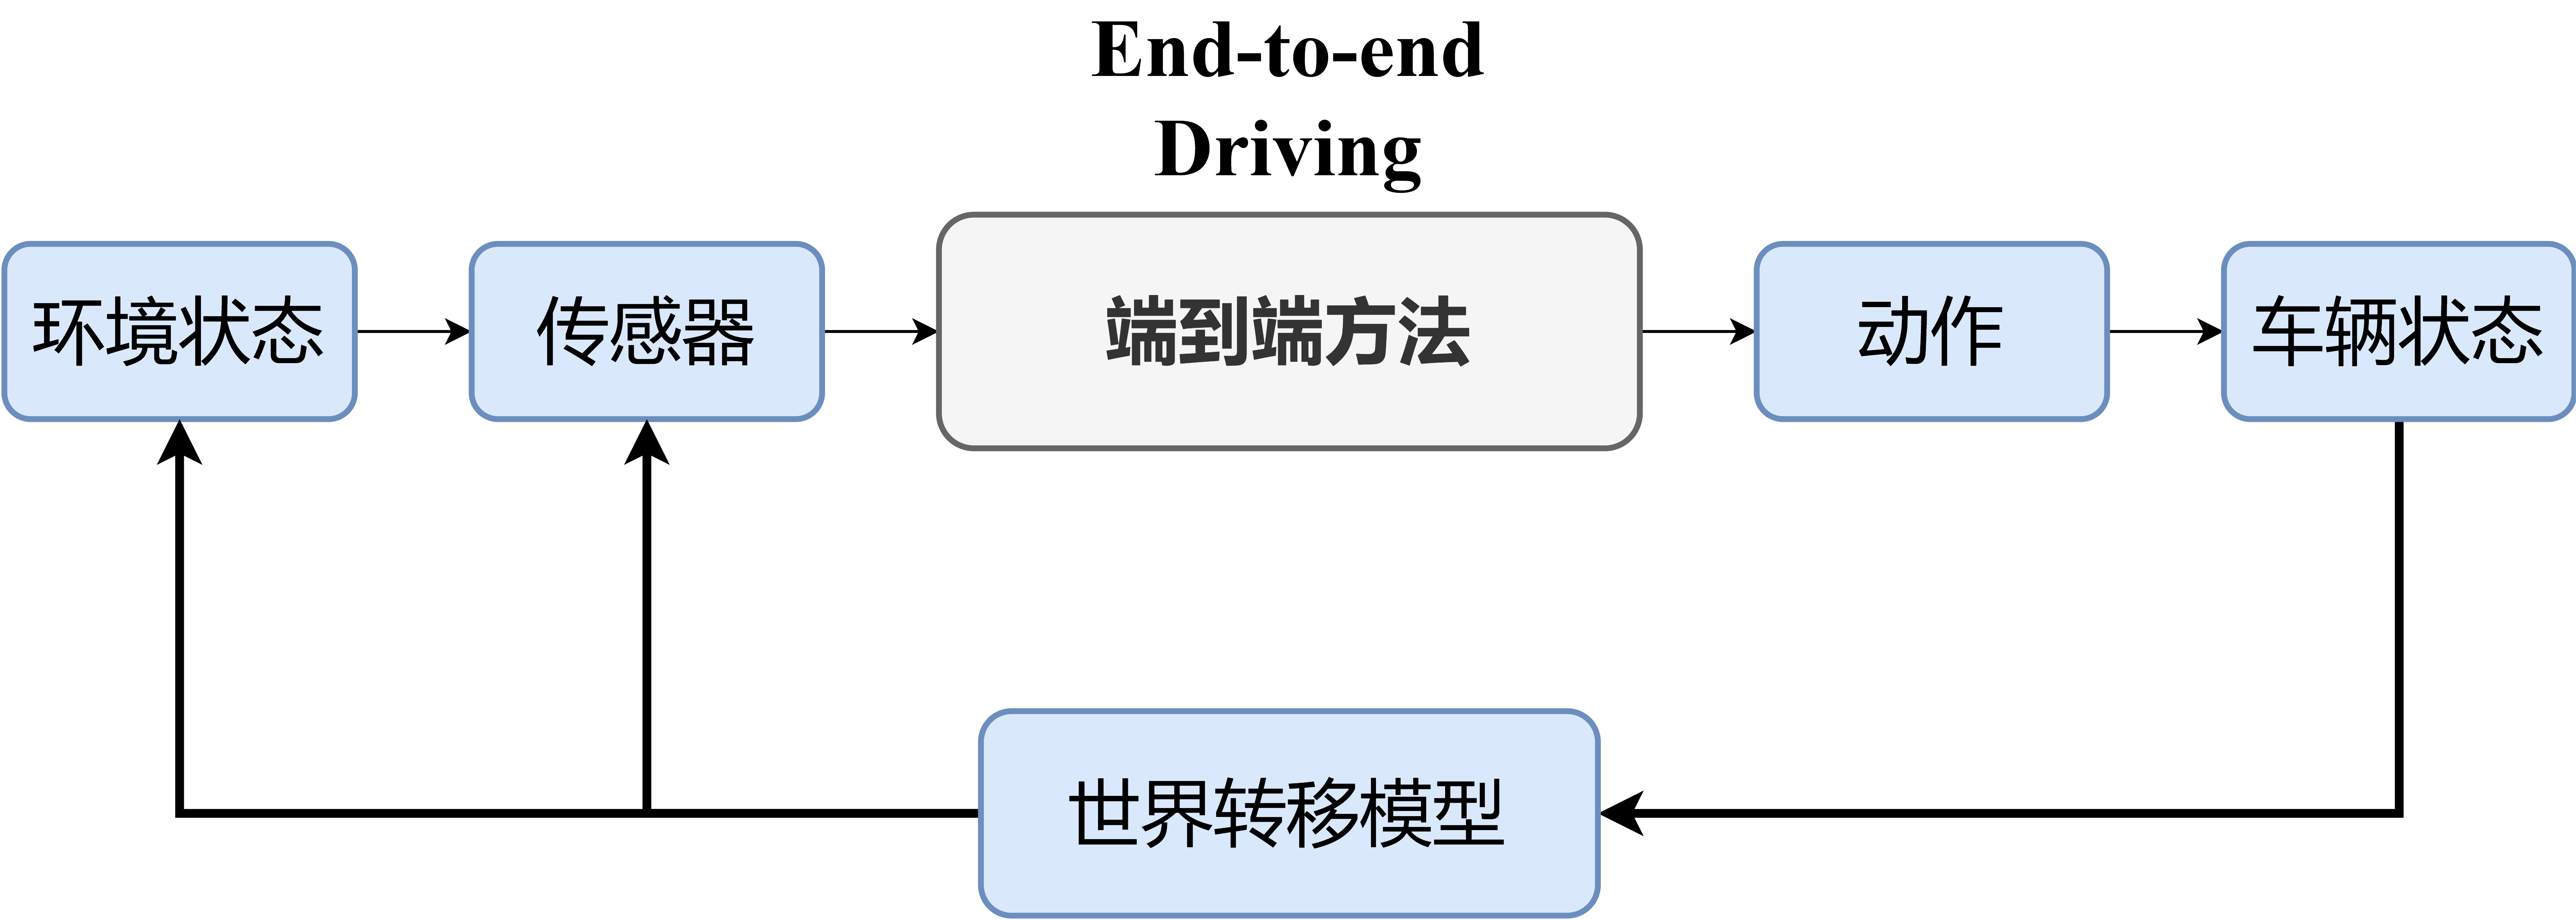
\includegraphics[width=1.0\textwidth]{images/chapter1/EndtoEnd_structure.png}
  \caption{端到端方法流程图}\label{端到端方法流程图} % label 用来在文中索引
\end{figure}

深度学习和强化学习的发展使得直接从原始的数据中提取高水平特征进行感知决策变成可能。深度学习起源于人工神经网络。早期研究人员提出了多层感知机的概念, 并且使用反向传播算法优化多层神经网络, 但是由于受到硬件等资源的限制, 神经网络的研究一直没有取得突破性进展。最近几年, 随着计算资源的性能提升和相应算法的发展, 深度学习在人工智能领域取得了一系列重大突破, 包括图像识别、语音识别、自然语言处理等。深度学习由于其强大的表征能力和泛化性能受到众多研究人员的关注, 相关技术在学术界和工业界都得到了广泛的研究与应用。

深度强化学习由数据驱动,不需要构造系统模型,具有很强的自适应能力。普林斯顿大学的Chen等使用深度学习算法, 根据摄像头采集的图像数据预测目标的距离, 同时输出操作指令\cite{2015DeepDriving}。斯坦福大学的Zhu等使用暹罗网络结构, 同时输入当前视角图像和目标物体图像, 并且使用残差网络模型提取特征。通过A3C(Asynchronous Advantage Actor-critic)算法进行训练, 成功控制小车在虚拟场景和现实场景中到达指定地点\cite{2016Target}。国内的Zhao等使用深度强化学习算法和注意力机制, 实现了智能驾驶领域车辆的高精度分类\cite{2017Deepzhao}。Zhu基于TORCS的真实物理变量, 使用高斯过程强化学习算法PILCO(Probabilistic Inference for Learning Control)离线训练控制器, 实现车道保持。同时以图像为输入, 使用深度学习算法感知环境信息, 预测本车距离车到中央线距离、偏航角、道路曲率等。最终将RL的控制策略和DL的特征预测结合, 实现基于图像的车道保持。

以上研究仅由大量的数据驱动而未单独考虑模型的影响,针对自动驾驶避障技术的模型问题,德克萨斯大学奥斯汀分校的Chen等提出“Learning to drive from a world on rails”的假设\cite{2021Learning},即车辆运动只与自身模型相关而与世界模型无关,采用世界模型与车辆模型解耦的方式建立一个前向模型来帮助改进自动驾驶策略;David Ha等提出生成循环神经网络以无监督的方式快速训练,通过压缩时空表征来模拟流行的强化学习环境\cite{2018Recurrent}。

%主要讲讲DQN
针对具体的深度强化学习算法,2012年,Lange等人最早在插槽赛车上使用深度强化学习算法并取得了良好的控制效果\cite{2012Autonomous}。2013年,由DeepMind团队提出的DQN(Deep Q-Network)算法利用深度卷积神经网络直接学习Atari2600种游戏的高维度图像,从输入中提取环境的高效描述,来近似最优动作-状态函数,从而习得成功策略\cite{2013DQN}。2015年,Hasselt等人发现传统的Q-learning和DQN方法都会普遍过高估计行为值函数Q值,存在过优化的问题,为了解决值函数过估计的问题,Hasselt提出了Double DQN方法,将行为选择和行为评估采用不同的值函数实现,降低了过估计的误差\cite{2015DDQN}。2016年,Wang提出Dueling DQN方法,把Q网络的结构显式地约束成跟动作无关的状态值函数$V(s)$与在状态$s$下各个动作的优势函数$A(s,a)$之和,使得DQN训练更容易,收敛速度更快,避免因为Q值的量级大而引起的结果不稳定问题\cite{2016DuelingDQN}。2017年,Zong等人使用深度确定性策略梯度DDPG算法对智能体的加速度和转向控制进行训练,以实现自主避障,并在开源赛车模拟器(TORCS)环境中进行了测试,结果表明通过一段时间自主学习,无人驾驶汽车能学会复杂的避障换道行为\cite{2017Obstacle}。该算法是将DQN和Actor-Critic算法相结合,使用深度神经网络来逼近值函数和策略函数,虽然,DDPG算法实现了连续状态、动作空间下的强化学习,然而算法参数并不易确定,其超参数往往必须针对不同的问题进行仔细设置才能获得良好的训练结果。

% Apollo
目前,一般的深度强化学习在商用领域仍未落地,当前的算法大多是采用深度强化学习进行端到端的路径规划,通过传感器输入的信息和先验地图信息输出轨迹信息,百度Apollo团队在2022年发布的ApolloRL平台\cite{2022ApolloRL},采用DRL作为自动驾驶车辆的轨迹输出,并用多种控制器如(MPC、LQR、PID)等对路径实现紧密跟踪,百度团队的做法对于深度强化学习在自动驾驶中的落地具有一定的借鉴作用。

随着研究的不断深入,深度强化学习算法在自动驾驶控制策略的应用范围越来越广,解决的问题也越来越复杂。这充分说明了深度强化学习算法应用于自动驾驶决策控制领域的可行性和有效性。本文在调研和分析相关文献的基础上基于深度强化学习算法设计自动驾驶决策控制算法,通过对比多种深度强化学习算法及其改进算法,验证在抽象环境与高维环境下深度强化学习算法的有效性和准确度。

\section{本文主要研究内容及章节安排} % 绪论、算法概览、两个仿真环境和改进的算法设计、结果、总结。

本文以DQN算法作为基础,探究DQN及其改进算法Double DQN和Dueling DQN在两种不同仿真环境(Highway-Env、Metadrive)中对自动驾驶决策及控制产生的效果。通过在仿真环境下的反复训练和学习,训练的模型在多种仿真环境下均具有较好的鲁棒性,证明了DQN及其改进算法在自动驾驶决策及控制方面的有效性和可行性。

第 1 章绪论。介绍了该课题的研究背景和意义,对强化学习在自动驾驶决策方面的发展现状进行了介绍,对深度强化学习特别是DQN算法的研究现状进行了详细的分析说明,在章节的最后通过分析总结参考文献得出了本文的研究方向和研究内容。

第 2 章强化学习相关算法理论分析。通过对强化学习算法原理的分析,引出了适用于无模型的 Q-learning 算法和 DQN 算法,同时,针对于DQN算法的不足和缺陷,介绍了Double DQN算法和Dueling DQN算法的原理,并对几种算法的适用场景进行了分析。

第 3 章基于DQN算法的自动驾驶避障算法设计。通过对两种仿真环境(Highway-Env、Metadrive)的分析和对比,介绍二者的状态值、动作值与奖励算法的详细情况。将DQN及其改进算法作用于两种仿真环境,同时改进Q网络的网络结构及超参数,使其完成自动驾驶决策和控制两方面的任务要求。

第 4 章实验验证。为了验证算法的可行性和有效性,进行了两种仿真环境中的仿真实验,并对具体的实验内容进行了分析与设计,对最后的实验结果进行了详细的分析与改进。

文章的最后进行了总结,对本文完成的主要工作和取得的主要成就进行了概述,对本文的创新点进行了阐述,同时指出了本文研究的不足和后续研究的重点内容。


% 在这里添加第二章、第三章……TeX 文件的引用
 %%
% The BIThesis Template for Bachelor Graduation Thesis
%
% 北京理工大学毕业设计(论文)第二章节 —— 使用 XeLaTeX 编译
%
% Copyright 2020-2021 BITNP
%
% This work may be distributed and/or modified under the
% conditions of the LaTeX Project Public License, either version 1.3
% of this license or (at your option) any later version.
% The latest version of this license is in
%   http://www.latex-project.org/lppl.txt
% and version 1.3 or later is part of all distributions of LaTeX
% version 2005/12/01 or later.
%
% This work has the LPPL maintenance status `maintained'.
%
% The Current Maintainer of this work is Huang Chenrui.
%%

\chapter{强化学习相关算法理论分析} % 强化学习算法理论、Q-learning、DQN、Double DQN、Dueling DQN

如图\ref{强化学习原理}所示,强化学习的基本原理在1.1节中已有提及,在此不再赘述。强化学习强调智能体与环境不断地交互,从而产生更多数据(状态和回报),并利用新的数据进一步改善自身的行为。智能体不会被告知在当前状态下,应该采取哪一个动作,只能通过不断尝试,依靠环境对动作的反馈改善自己的行为。经过数次迭代后,智能体最终能学到完成相应任务的最优动作(策略)。

本章通过对强化学习以及相关算法的理论分析,对基于值函数(Value Based)的Q-learning算法及DQN算法进行详细介绍,对DQN算法及其改进算法的优劣进行比较,选择最适合解决自动驾驶决策控制的方法。

\section{强化学习算法} % 算法的组成、选择基于值函数方法的原因、算法的求解过程。

强化学习包括智能体和环境两大对象。智能体又称为学习者或玩家,环境是指与智能体交互的内部。智能体由策略、值函数、模型三个组成部分中的一个或多个组成。下文将介绍强化学习智能体的各个组成部分与强化学习问题求解的目标,由此引出基于值函数的强化学习方法。

\subsection{强化学习算法的组成} % 谈谈为什么要选择基于值函数的方法。

(1)策略:策略是决定智能体行为的机制,是状态到行为的映射,用$\pi(a|s)$表示,它定义了智能体在各个状态下的各种可能的行为及概率。
\begin{equation}\label{pi}
    \pi(a|s) = P(A_t = a | S_t = s)
\end{equation}
策略分为两种,确定性策略和随机性策略。确定性策略根据智能体具体状态输出一个确切的动作,而随机性策略根据状态输出智能体每个动作的概率,输出值为一个概率分布。
一个策略完整定义了智能体在各个状态下的各种可能的动作及其概率大小。策略仅和当前状态有关,与历史信息无关。策略就是用来描述各个不同状态下执行各个不同行为的概率,同一时刻某一确定的策略是静态的,与时间无关,但是智能体可以随着时间更新策略。

(2)值函数:值函数代表智能体在给定状态下采取某个行为的好坏程度。这里的好坏用未来的期望回报表示,而回报和采取的策略有关,所有值函数的估计都是基于给定的策略进行的。值函数(或称为回报)用$G_t$表示,也称为“收益”或“奖励”。
\begin{equation}\label{G_t}
    G_t = R_{t+1} + \gamma R_{t+2} + \gamma^2 R_{t+3} + \dots = \sum_{k=0}^\infty \gamma^k R_{t+k+1}
\end{equation} 
其中折扣因子$\gamma$(衰减系数)体现了未来的回报在当前时刻的价值比例,在$k+1$时刻获得的回报$R$在$t$时刻体现出的价值是$\gamma^k R$。$\gamma$接近0表示趋向于当前利益;$\gamma$接近1表示偏向于长远期的利益。

值函数分为状态值函数与状态行为值函数,二者都与回报有关。

状态值函数$V_{\pi}(s)$表示从状态$s$开始,遵循当前策略$\pi$所获得的期望回报。
\begin{equation}
    \begin{aligned}
        V_{\pi}(s) &= E_{\pi}[G_t | S_t = s]\\
                     &= E_{\pi}[R_{t+1} + \gamma R_{t+2} + \gamma^2 R_{t+3} + \dots | S_t = s]\\
    \end{aligned}
\end{equation}

值函数的另一个类别是状态行为值函数$Q_{\pi}(s,a)$,也称为行为值函数。该函数表示针对当前状态$s$执行某一具体行为$a$后,继续执行策略$\pi$所获得的期望回报;也表示遵循策略$\pi$时,对当前状态$s$执行行为$a$的价值大小。
\begin{equation}
    \begin{aligned}
        Q_{\pi}(s,a) &= E_{\pi}[G_t | S_t = s, A_t =a]\\
                     &= E_{\pi}[R_{t+1} + \gamma R_{t+2} + \gamma^2 R_{t+3} + \dots | S_t = s, A_t =a]\\
    \end{aligned}
\end{equation}

(3)模型:在强化学习任务中,模型是智能体对环境的一个建模。环境模型至少要解决两个问题,一是预测状态转移概率$P_{ss^{'}}^a$,即预测在状态$s$上采取行为$a$后,下一个状态$s^{'}$的概率分布;二是预测在状态$s$上采取行为$a$后可能获得的立即回报$R_s^a$。
\begin{equation}
    \begin{aligned}
        & P_{ss^{'}}^a = P(S_{t+1} = s^{'} | S_t = s, A_t = a) \\
        & R_s^a = E[R_{t+1} | S_t = s, A_t = a] \\
    \end{aligned}
\end{equation}
根据智能体在与环境交互的过程中是否建立环境的模型,强化学习可以分为两个大类,即有模型方法和无模型方法。
一般的模型已知问题,就是智能体获得了确切的状态转移概率$P_{ss^{'}}^a$和回报$R_s^a$。

在后续章节的仿真环境介绍中,由于车辆的决策控制较难采用已知模型(如动力学模型、运动学模型)进行刻画,故均使用“无模型方法”的假设,即智能体在整个训练过程中不需要对环境模型进行建模,直接使用学习得到的经验进行策略的优化。

根据以上三点概念,可以通过建立状态值估计的方法或建立策略估计的方法来解决强化学习问题。基于值函数的方法在求解强化学习的目标时只估计状态值函数,不估计策略函数,最优策略函数在对值函数进行迭代求解时,通过状态值函数间接得到。针对自动驾驶避障问题,由于我们较难估计车辆状态与行为之间的映射(即策略函数),但可以估计车辆在采取某个动作时,车辆状态发生的变化和环境回报(即状态值函数),所以采取基于值函数的方法更加符合解决自动驾驶避障问题所需要达成的目标。

\subsection{强化学习算法的求解} % 谈谈求解强化学习算法需要什么(仿真环境[抽象问题] + 算法网络)           % TODO:这里要不要绘制一个马尔科夫决策链放附录?

求解强化学习问题的目标是求解每个状态下的最优策略,即在运行过程中接收的累计回报最大。为了获取更高的回报,智能体在进行决策时要考虑立即回报,也要考虑后续状态的回报。解决强化学习问题一般需要两步,将实际场景抽象成一个数学模型,然后去求解这个数学模型,找到使得累计回报最大的解。

第一步:构建强化学习的数学模型——马尔科夫决策(Markov Decision Process, MDP)\cite{monahan1982state}模型。

不论涉及的智能体结构、环境和交互细节多么复杂,此类交互问题都能简化为三个信号:智能体的行为、环境的状态、环境反馈的回报。具体到实验中,便是仿真环境根据智能体做出的行为产生的回报和改变的状态。马尔科夫决策模型可以有效表示实际的强化学习问题,这样解决强化学习问题的问题就转化为求解马尔科夫决策模型的最优解。

第二步:求解马尔科夫决策模型的最优解。

求解马尔科夫决策问题,是指求解每个状态下的行为,使得累计回报最大。对于环境已知的情况可以选用基于模型的方法如动态规划法;基于未知的情况选择无模型方法如时序差分法;对于状态空间、动作空间连续的场景可以采用值函数逼近法等等。根据2.1.1节的分析,如何求解马尔科夫决策模型便是具体的算法与网络结构,下文将对基于值函数(Value Based)的Q-learning算法及DQN算法进行详细介绍。

\section{Q-learning算法} % 先讲时序差分TD,再讲Q-learning。

在介绍Q-learning算法之前,首先对时序差分方法进行简单的介绍。时序差分学习最早由A.Summuel在跳棋算法中提出,1988年,Sutton证明了时序差分方法在最小均方误差(MSE)上的收敛性\cite{1998Reinforcement},之后时序差分方法被广泛应用在无法产生完整轨迹的无模型强化学习问题上。时序差分(TD)方法是无模型方法,无法获得当前状态的所有后续状态及回报,仅能通过采样学习轨迹片段,用下一状态的预估状态价值更新当前的状态价值。

Q-learning算法属于离线策略时序差分(TD)问题,最早由Watkins和Dayan在1992年提出\cite{1992Technical},其任务是通过不断地学习,不断的更新状态-动作值函数$Q(s,a)$,从而得出最优策略。根据2.1.2节中所提到的,求解强化学习问题的目标是求解每个状态下的最优策略,Q-learning算法在更新一个状态-动作值函数(以下简称Q值)时,采用的不是遵循当前策略(行为策略$\mu$)的下一个状态-动作对的Q值,而是待评估策略(目标策略$\pi$)产生的下一个状态-动作对的Q值。更新公式如下:
\begin{equation}\label{Q-learning}
    Q(S_t, A_t) \gets Q(S_t, A_t) + \alpha (R_{t+1}+\gamma Q(S_t, A^{'}) - Q(S_t, A_t))
\end{equation}
其中$\alpha$称为学习率,$\gamma$称为折扣因子,TD目标$R_{t+1}+\gamma Q(S_t, A^{'})$是基于目标策略$\pi$产生的行为$A^{'}$得到的Q值和一个立即回报的和。在Q-learning算法中,行为策略$\mu$是基于原始策略的$\epsilon$-贪心策略,保证取得经历足够丰富的新状态。目标函数$\pi$是单纯的贪心策略,通过最大化TD目标来保证策略最终收敛到最佳策略。

Q-learning算法处理有限的状态空间与有限的动作空间的问题,状态值和动作放在Q表中,值函数能够表示为一个数组。但在实际情况下,强化学习面临的问题的状态空间往往是连续的,无法用表格的方法准确列出每一种状态对应的Q值大小,故需要进行对Q值进行非线性的逼近。下文的DQN就属于这样的方法。无论是Q-learning或是DQN,均采用了目标策略$\pi$产生的下一个状态-动作对的Q值对原有的Q值进行更新,这是时序差分法的一般思想。

Q-learning的算法流程如下:

\begin{algorithm}[H]  
	\caption{Q-learning算法}%算法名字
	\KwIn{环境$E$,状态$S$,动作$A$,折扣因子$\gamma$,学习率$\alpha$,初始化行为值函数$Q(s,a)=0$}%输入参数
	\For{k = 0,1,2,\dots,m}{
		初始化状态s\;
		\For{t=0,1,2,\dots}{
            在$E$中通过$\pi$的$\epsilon$-贪心策略采取行为$a$\;
            $r$,$s^{'}=$在$E$中执行动作$a$产生的回报和转移的状态\;
            $Q(S_t, A_t) \gets Q(S_t, A_t) + \alpha (R_{t+1}+\gamma Q(S_t, A^{'}) - Q(S_t, A_t))$\;
            $s \gets s^{'}$\;
        }
	}
    $\pi^{*}(s) = \arg \max_{a \in A} Q(s,a)$\;
    \KwOut{最优策略$\pi^{*}$}%输出
\end{algorithm}

\section{DQN算法} % DQN网络图+较为具体的实现。

DQN(Deep Q-Network)算法是建立传统强化学习算法Q-learning的基础上的时序差分算法,Q-learning是离线策略时序差分法,使用$\epsilon$贪心策略产生数据,利用查表法对行为值函数(Q值)进行预测,TD目标是$R_{t+1}+\gamma Q(S_t, A^{'})$。DQN算法在传统强化学习Q-learning的基础上,主要对其精确的查表法做了近似拟合,同时通过引入深度学习网络,对网络结构和参数更新做出了如下改进。

(1)DQN使用深度神经网络从原始数据中提取特征,近似行为值函数(Q值)。

当状态空间很大且连续时,无法使用查表法来求解每个状态的价值,此时可以考虑“离散”状态空间的方法来减少算力。在“离散”状态空间中,使用深度神经网络来表示行为值函数是常见的方法。对于深度神经网络,其参数是每层网络的权重及偏置,用$\theta$表示,对值函数的更新等价于对参数$\theta$的更新。DQN神经网络结构如图\ref{DQN神经网络结构}所示。

DQN神经网络结构是三个卷积层和两个全连接层。输入为经过处理的4个连续的84$\times$84的图像,经过卷积层和两个全连接层输出包含每一个动作的Q值向量。DQN网络将高维的状态输入转换为低维的动作输出,即将图像输入转换为动作输出。利用深度神经网络实现了数据的降维。

\begin{figure}[htbp]
    \vspace{13pt} % 调整图片与上文的垂直距离
    \centering
    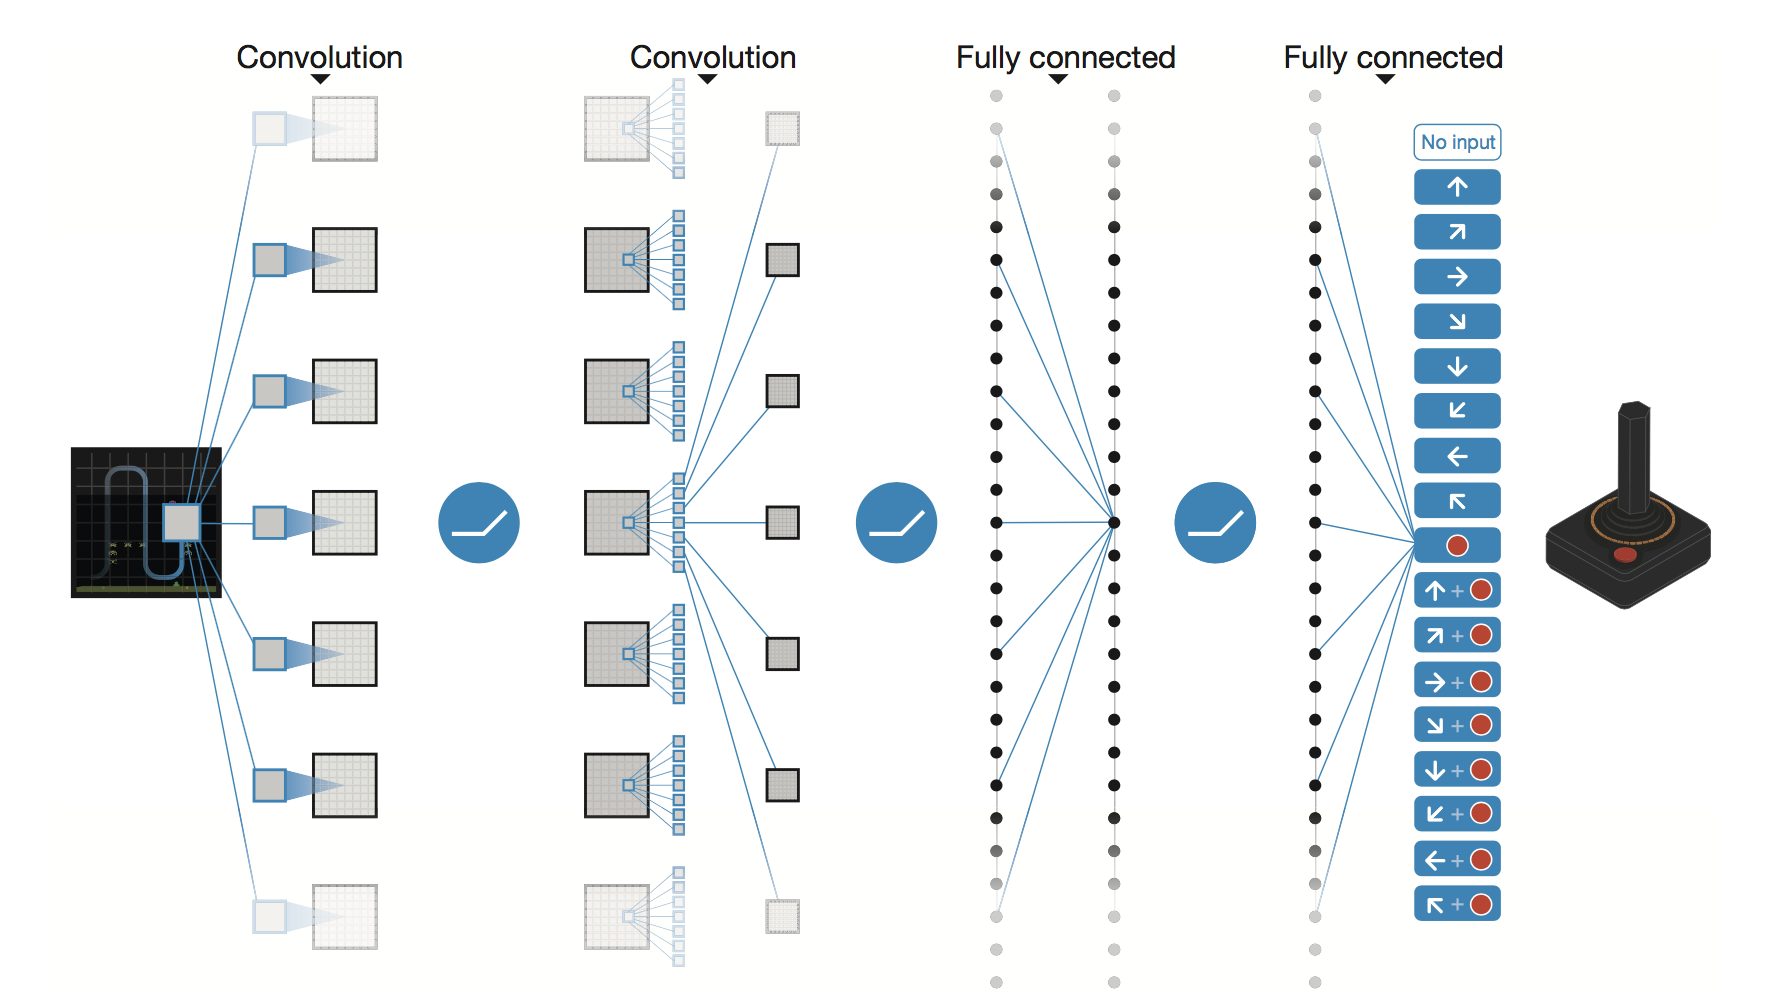
\includegraphics[width=0.73\textwidth]{images/chapter2/DQN_model.png}
    \caption{DQN神经网络结构}\label{DQN神经网络结构} % label 用来在文中索引
\end{figure}

(2)DQN使用经历回放训练强化学习。

在使用深度神经网络进行行为值函数(Q值)近似时,如果不对训练数据做处理,直接将当前时刻的信息进行学习训练,学习效果会出现较大偏差。由于使用神经网络的前提是数据之间独立同分布,而强化学习过程中,数据是通过与环境交互产生的,相邻数据之间高度相关。如果智能体在很长一段时间均学习相同环境下的数据,在接收到另一环境的数据后,参数会出现不稳定与大范围波动发散,求解无法收敛。针对这一问题,DQN采用“经验回放”的方法进行解决。

\begin{figure}[htbp]
    \vspace{13pt} % 调整图片与上文的垂直距离
    \centering
    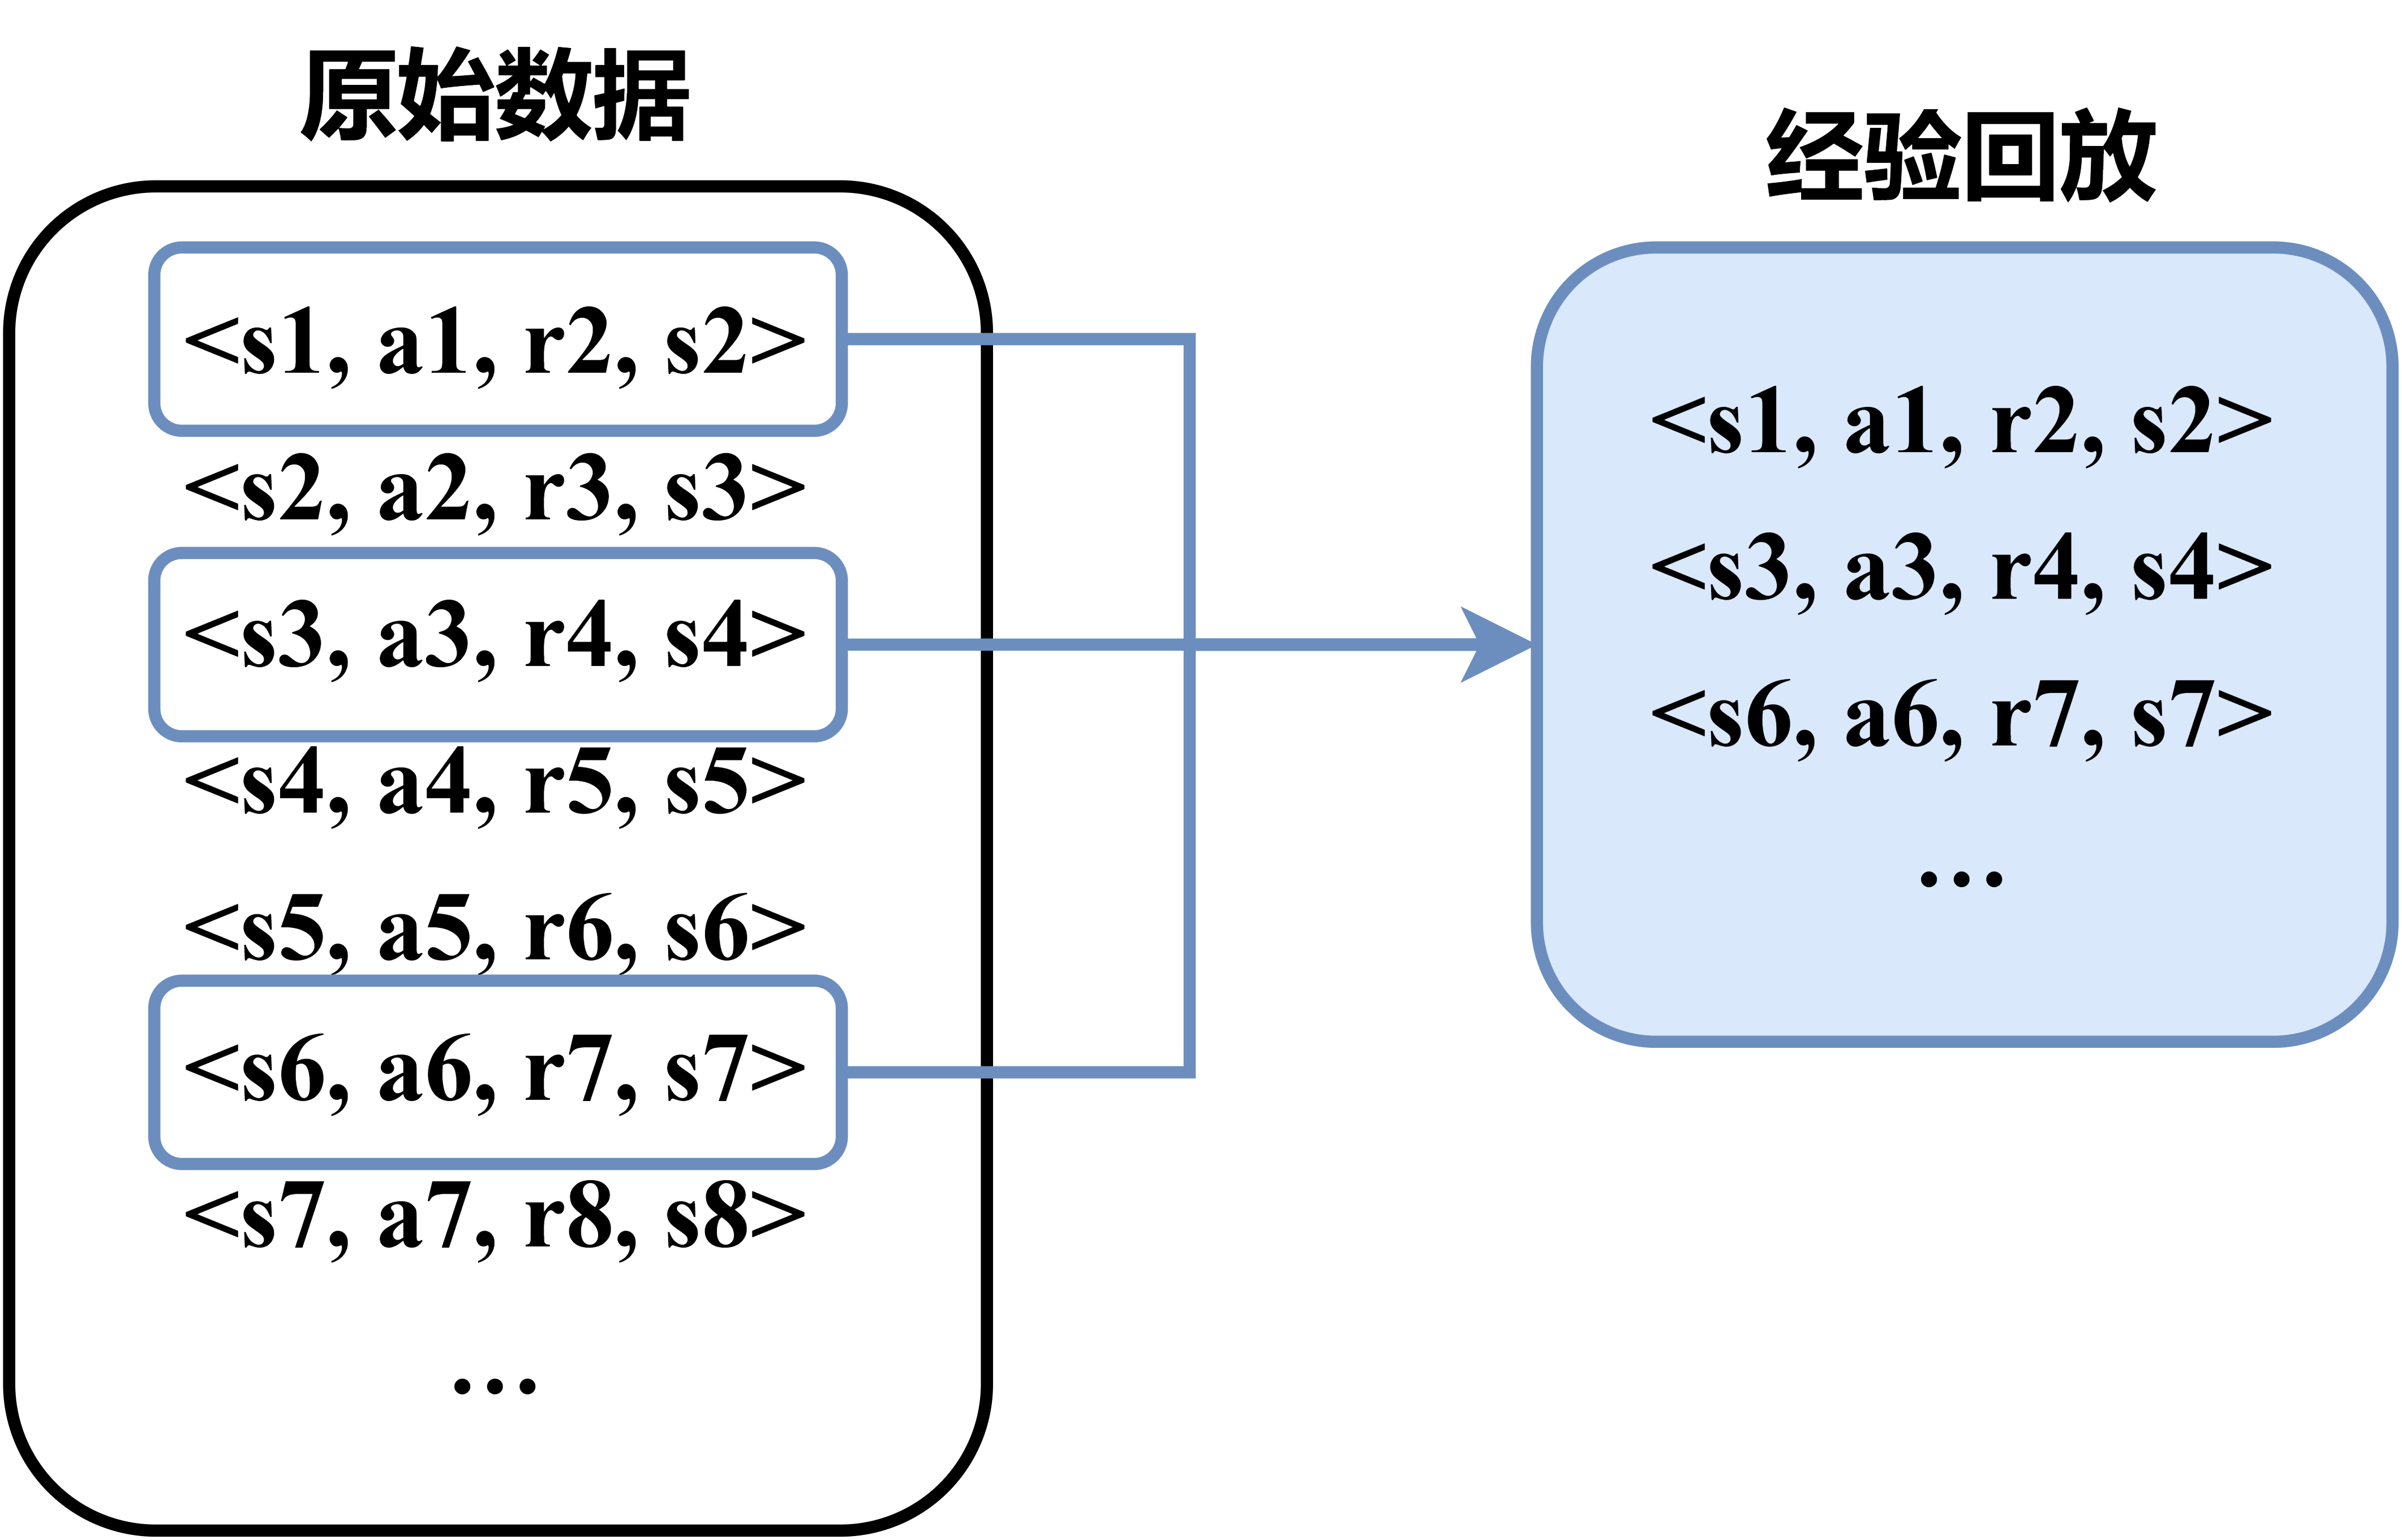
\includegraphics[width=0.63\textwidth]{images/chapter2/Experience_Replay.png}
    \caption{经验回放}\label{经验回放} % label 用来在文中索引
\end{figure}

经验回放最早由Long Ji Lin在1993年提出\cite{1992Reinforcement},如图\ref{经验回放},它在强化学习中是这样实现的:智能体跟环境不断交互,将在环境中积累的数据存储到记忆库中。首先对环境做出探索并将<本时刻状态、行为、奖励、下一时刻状态>($<s_1, a_1, r_2, s_2>$)作为一个事件对进行存储,每一次对神经网络中的参数进行更新时,利用均匀随机采样的方法从数据库中抽取数据,通过抽取的数据对神经网络进行训练。因为经验回放的样本是随机抽取,每次用于训练的样本不再是连续的数据,打破了数据的关联,由此可以满足神经网络的假设要求。

(3)DQN使用单独的目标网络处理TD偏差。

与式\ref{Q-learning}类似,DQN更新神经网络的参数$\theta$采用的是梯度下降法。更新公式如下:
\begin{equation*}
    \theta_{t+1} = \theta_t + \alpha (r + \gamma \max_{a^{'}} Q(s^{'}, a^{'}; \theta_t) - Q(s, a; \theta_t))\nabla   Q(s, a; \theta_t)
\end{equation*}

但如(2)中提及,行为值函数($Q(s, a; \theta_t)$)和TD目标值函数($r + \gamma \max_{a^{'}} Q(s^{'}, a^{'}; \theta_t)$)产生的数据需要避免关联性。为解决上述问题,DQN引入两个神经网络,一个网络固定参数专门用来产生TD目标,称为TD网络。另一个网络专门用来评估策略更新函数,逼近值函数,称为行为值函数(Q值)逼近网络。两个网络参数的更新速率不一致,用于行为值函数(Q值)逼近的网络参数每一步都更新;用于计算TD目标值的网络参数每隔固定的步数更新一次,期间保证不变。于是得到以下DQN网络的更新公式:
\begin{equation}\label{DQN}
    \theta_{t+1} = \theta_t + \alpha (r + \gamma \max_{a^{'}} Q(s^{'}, a^{'}; \theta_t^{-}) - Q(s, a; \theta_t))\nabla   Q(s, a; \theta_t)
\end{equation}

综合上述三点改进,DQN算法将经验回放和设置单独的目标网络两个方面对Q-learning方法进行改善,使其对于更加复杂的问题和大规模神经网络更加稳定和容易收敛,DQN的算法流程如下:

\begin{algorithm}[H]  
	\caption{DQN算法}%算法名字
	\KwIn{环境$E$,状态$S$,动作$A$,折扣因子$\gamma$,学习率$\alpha$}%输入参数
	初始化经验回放库D并定义容量N\;
    随机初始化网络参数$\theta$,用$\theta$初始化主网络$Q(; \theta)$\;
    随机初始化网络参数$\theta^{-}=\theta$,用$\theta^{-}$初始化TD网络$Q(; \theta^{-})$\;
    \For{k = 0,1,2,\dots,m}{
		初始化状态s\;
		\For{t=0,1,2,\dots}{
            在$E$中通过主网络的$\epsilon$-贪心策略采取行为$a$(以$\epsilon$概率随机选择任一随机动作,以$1-\epsilon$概率选择行为值函数最大的动作,即$a = \arg \max_{a \in A} Q(s,a; \theta)$\;
            在$E$中执行动作$a$,返回奖励$r$,和下一时刻状态$s^{'}$\;
            将当前事件对$<s,a,r,s^{'}>$存入经验回放库D中\;
            从经验回放库D中随机采样$n$个数据,进行如下算法更新:\
            $
                q_{target} = 
                \begin{cases}
                    r , &end\\
                    r + \gamma \max Q(s^{'},a;\theta^{-} ), &else
                \end{cases}
            $
            \\
            $
                q_{next} = Q(s,a;\theta)
            $
            \\
            $Loss = (q_{target} - q_{next})^2$\;
            对于主网络参数$\theta$使用$Loss$进行梯度下降法更新网络参数$\theta$\;
            每隔X步更新一次TD网络,$\theta^{-} \gets \theta$\;
        }
	}
    \KwOut{最优网络参数$\theta$}%输出
\end{algorithm}

\section{改进的DQN算法} % DDQN、Dueling DQN的具体讲解和公式阐明。

由式\ref{Q-learning}与式\ref{DQN}可知,不论是Q-learning还是DQN,值函数的更新公式中均有最大化操作,通过最大化值函数网络的操作来选择行为。通过最大化值函数网络的操作来选择行为并进行评估,整体上使得估计的值函数比真实的值函数大,并且误差会随着动作空间的增加而增加。此时产生的过估计量往往是非均匀的,故此时值函数的过估计就会影响到最优决策,导致最终选择一个次优的动作。

为了解决DQN的不足,Double DQN和Dueling DQN分别从网络的更新策略和网络的结构上做出了改进。

\subsection{Double DQN算法}% 主要是公式的差异。

为了解决值函数过估计的问题,Hasselt提出了Double DQN方法\cite{2015DDQN}。传统DQN中,选择行为指的是选择一个动作a,使其满足$a = \arg \max_a Q(s',a; \theta{-})$;评估行为指的是利用$a$构建TD目标$q_{target}$,$q_{target} = r + \gamma \max Q(s^{'},a; \theta^{-})$,选择行为和评估行为用的是同一个Q网络及其网络参数。

Double DQN分别采用不同的值函数来实现动作选择和动作评估。针对于传统DQN,由于传统DQN已经存在两个网络(主网络和TD网络),因此不需要改变DQN的网络结构,只需要改变DQN的参数更新策略。Double DQN和DQN的区别在于:

(1)首先使用主网络选择动作。
\begin{equation*}
    a = \arg \max_a Q(s',a; \theta)
\end{equation*}

(2)其次使用TD网络找到该动作对应的Q值,构成TD目标。
\begin{equation*}
    \begin{aligned}
        q_{target} &= r + \gamma Q(s^{'}, a; \theta^{-})\\
                  &= r + \gamma Q(s^{'}, \arg \max_a Q(s',a; \theta); \theta^{-})
    \end{aligned}
\end{equation*}

此时构成的$q_{target}$在TD网络中不一定是最大的,但是该值是通过每步更新的主网络选取的最优动作,可以在一定程度上避免选到被高估的次优行为。Double DQN的其余流程均与DQN相似,故算法流程不再赘述。

\subsection{Dueling DQN算法}% 主要是结构图的表示。

在许多基于视觉感知的深度强化学习的任务中,不同的状态对应的值函数Q(s,a)是不同的,但是在某些状态下,值函数的大小与动作无关。Baird在1993年提出将Q值分解为价值(Value)和优势(Advantage)\cite{1993Advantage},即$Q(s,a) = V(s) + A(s,a)$。$V(s)$是在$s$状态下所有行为值函数(Q值)关于行为概率的期望,即所有可能行为对应的Q值乘以该行为所对应的概率之和。$A(s,a)=Q(s,a)-V(s)$,表示行为值函数相比于当前状态值函数的优势,即在这个状态下各个动作的优劣程度。

基于Baird的思想,将DQN用于竞争网络,就有了Dueling DQN算法的原理,图\ref{DuelingDQN网络结构}清晰地给出了Dueling DQN和DQN的网络结构差异。

\begin{figure}[htbp]
    \vspace{13pt} % 调整图片与上文的垂直距离
    \centering
    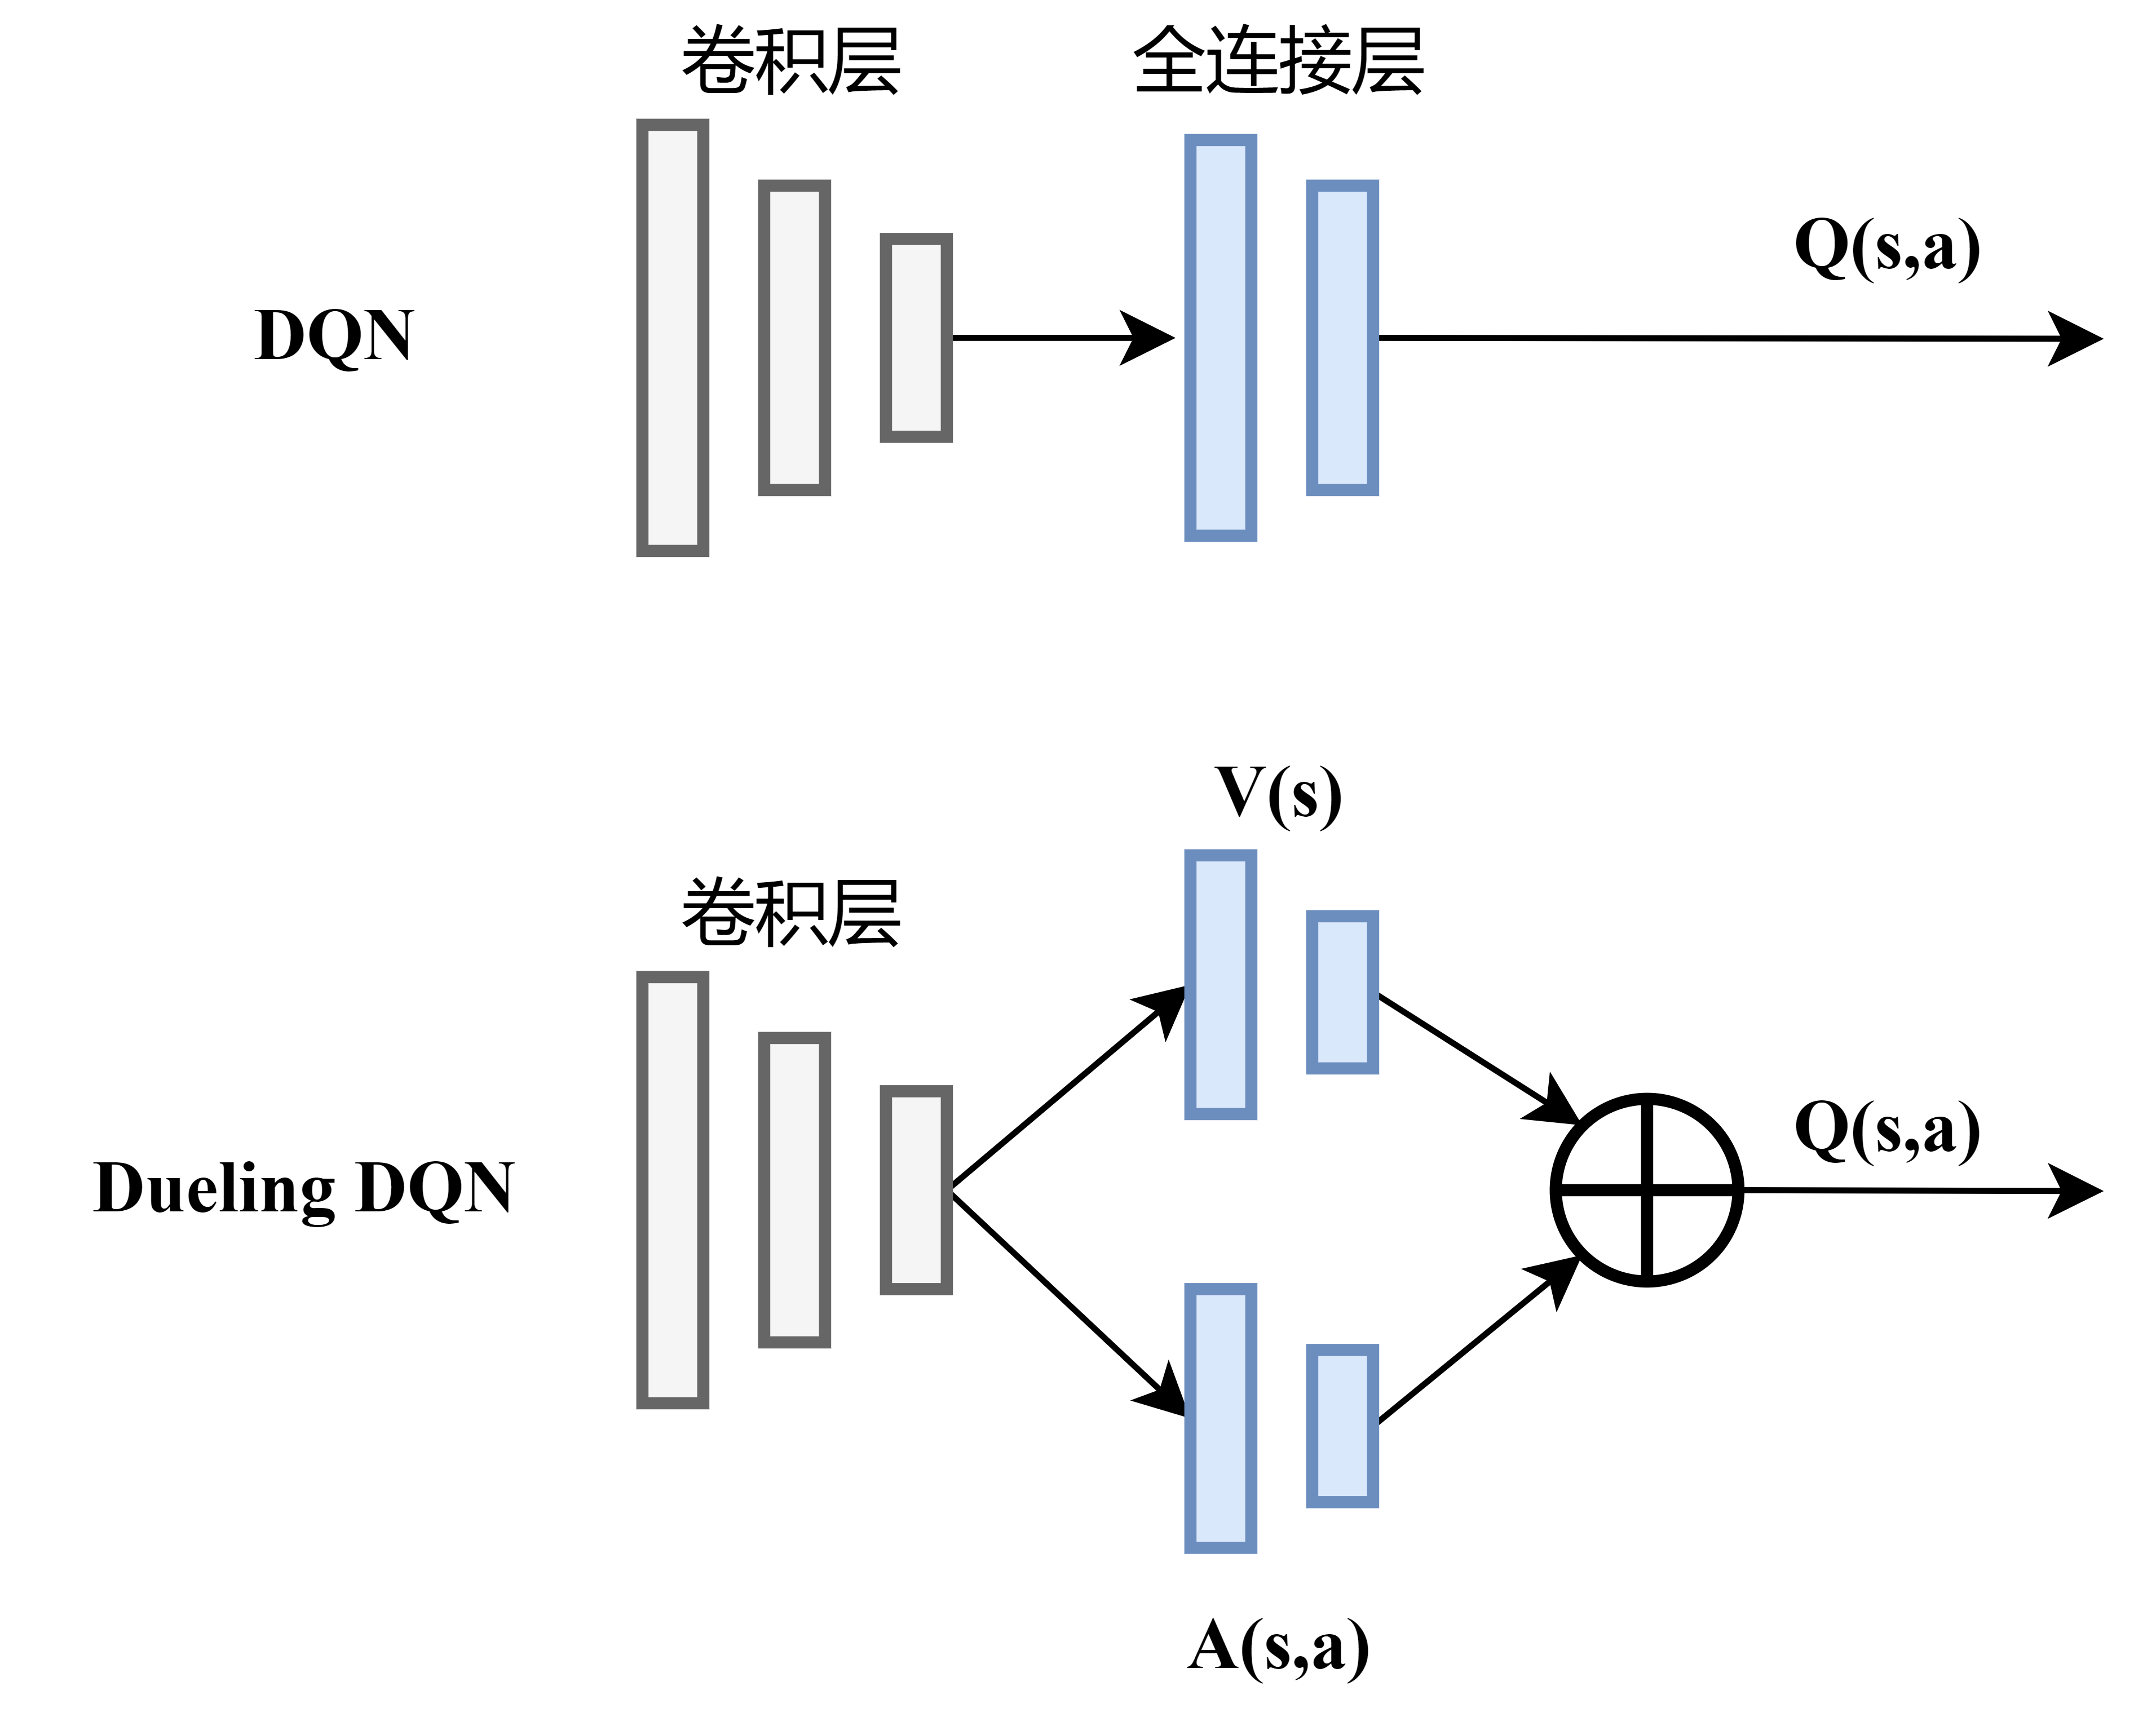
\includegraphics[width=0.63\textwidth]{images/chapter2/Dueling_DQN.png}
    \caption{DuelingDQN网络结构}\label{DuelingDQN网络结构} % label 用来在文中索引
\end{figure}

Dueling DQN将卷积层提取的抽象特征分流到两个支路上,两个支路所采用的全连接层结构相同。两个支路分别输出状态值函数$V(s)$和优势值函数$A(s,a)$,聚合函数将两个支路合并为Q函数:
\begin{equation*}
    Q(s,a;\alpha,\beta) = V(s;\beta) + A(s,a;\alpha)
\end{equation*}
但此式存在一个无法识别的问题,在确定的Q下,V和A有无数可能,故需要对A值做出限定,强制令所有选择贪婪动作的优势函数为0(认为没有比选择贪婪动作的方法更优的选项了)。添加约束条件,此时Dueling DQN的行为值函数为:
\begin{equation}
    Q(s,a;\alpha,\beta) = V(s;\beta) + A(s,a;\alpha) - \max_{a^{'} \in A}A(s,a^{'};\alpha)
\end{equation}

在实际中,一般使用优势函数的平均值代替上述最优值,虽然平均值改变了优势函数的值,但它可以保证缩小Q值的范围,去除多余的自由度,从而提高算法的稳定性。
\begin{equation}
    Q(s,a;\alpha,\beta) = V(s;\beta) + A(s,a;\alpha) - \frac{1}{\left | A \right | } \sum_{a^{'} \in A}A(s,a^{'};\alpha)
\end{equation}

由于Dueling DQN与传统DQN有相同的输入输出,只需要改变网络结构和前向传播的公式,除此之外算法的处理流程和DQN是相同的。

\section{本章小结}% 讲一下要用DQN、DDQN和Dueling DQN来干一些事情。

本章介绍了强化学习算法的组成及其马尔科夫决策模型的求解,通过对基于值函数(Value Based)的Q-learning算法及DQN算法的详细分析,由于自动驾驶决策控制任务无法进行精确的“查表”预知,需要进行神经网络的拟合,故采取基于DQN及其改进算法Double DQN和Dueling DQN算法完成自动驾驶决策控制任务。同时,根据输入数据的抽象程度,下一章节将对三种DQN算法进行决策与控制方面的设计与探究,从而得到DQN及其改进算法的对比实验效果。

 %%
% The BIThesis Template for Bachelor Graduation Thesis
%
% 北京理工大学毕业设计(论文)第三章节 —— 使用 XeLaTeX 编译
%
% Copyright 2020-2021 BITNP
%
% This work may be distributed and/or modified under the
% conditions of the LaTeX Project Public License, either version 1.3
% of this license or (at your option) any later version.
% The latest version of this license is in
%   http://www.latex-project.org/lppl.txt
% and version 1.3 or later is part of all distributions of LaTeX
% version 2005/12/01 or later.
%
% This work has the LPPL maintenance status `maintained'.
%
% The Current Maintainer of this work is Huang Chenrui.
%%

\chapter{基于DQN算法的自动驾驶避障算法设计}

在第2章的分析中,DQN、Double DQN和Dueling DQN能够完成自动驾驶决策控制任务。本章将结合Highway-Env与Metadrive两种仿真环境,设计决策器与控制器,分别探究在抽象的数据输入与具体的数据输入的情况下,DQN及其改进算法对自动驾驶车辆决策与控制任务的效果和不同算法作用下的对比实验,从而满足功能需求。

\section{基于DQN算法的决策器设计}\label{3.1基于DQN算法的决策器设计} % 3.1 决策任务

\subsection{仿真环境}\label{3.1.1仿真环境}

Highway-Env是一个用于自动驾驶决策的最小仿真环境\cite{highway-env},它包含了自动驾驶决策任务的环境集合。对强化学习而言,Highway-Env包含了强化学习所需要的状态(state)、动作(action)和奖惩值(reward)设计。Highway-Env的仿真效果如图\ref{highway-env}所示,在这项任务中,自我车辆(ego-vehicle)正在一条多车道高速公路上行驶,该高速公路上存在其他车辆。智能体的目标是在避免与邻近车辆发生碰撞的同时达到高速,将车辆保持在最下方的道路行驶也会获得奖励。

\begin{figure}[htbp]
    \vspace{13pt}
    \centering
    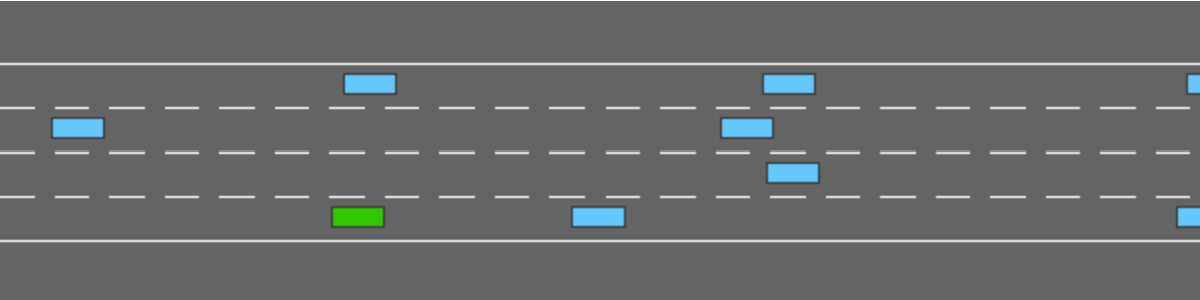
\includegraphics[width=0.73\textwidth]{images/chapter3/highway-env.png}
    \caption{highway-env仿真界面}\label{highway-env} % label 用来在文中索引
\end{figure}  

本文采用Highway-Env进行自动驾驶决策任务的设计,智能体(自我车辆)根据周围车辆的环境情况,获取环境反馈的奖惩值函数,通过执行决策行为间接控制车辆避障。因此,首先需要明确Highway-Env的状态、动作和奖励函数设计。

\subsubsection{Highway-Env的状态值设计}

在Highway-Env中有一系列的数据状态集合,针对自动驾驶避障问题,应当获取Kinetmatics的状态函数。Kinematics的状态是一张$V \times F$的表格,如表\ref{Kinetmatics状态表格}所示,$V$表示用户定义的车辆数量,$F$表示每个车辆的特征。第一列的$Vehicle$参数表示在当前画面中是否出现该车辆,如出现该车辆,则$Vehicle$值为1,否则为0。剩余的数值是车辆的坐标和速度,由于考虑的是自我车辆(ego-vehicle)的避障,所以环境中的其他车辆的坐标和速度均是相对于自我车辆的数值。

\begin{table}[htbp]
    % \vspace{13pt} % 调整图片与上文的垂直距离
    \caption{Kinetmatics状态表格}\label{Kinetmatics状态表格}
    \centering
    \renewcommand\arraystretch{1.5}
    \setlength{\tabcolsep}{7mm}{
    \begin{tabular}{|c|cccc|}
    \hline
    Vehicle     & \multicolumn{1}{c|}{$x$}  & \multicolumn{1}{c|}{$y$}  & \multicolumn{1}{c|}{$v_x$} & $v_y$ \\ \hline
    ego-vehicle & \multicolumn{1}{c|}{$x_{ego}$}   & \multicolumn{1}{c|}{$y_{ego}$}   & \multicolumn{1}{c|}{$v_{xego}$}      &  $v_{yego}$     \\ \hline
    vehicle 1   & \multicolumn{1}{c|}{$x_1$} & \multicolumn{1}{c|}{$y_1$} & \multicolumn{1}{c|}{$v_{x1}$}   & $v_{y1}$   \\ \hline
    vehicle 2   & \multicolumn{1}{c|}{$x_2$} & \multicolumn{1}{c|}{$y_2$} & \multicolumn{1}{c|}{$v_{x2}$}   & $v_{y2}$   \\ \hline
    $\dots$     & \multicolumn{4}{c|}{$\dots$}                                                           \\ \hline
    vehicle n   & \multicolumn{1}{c|}{$x_n$} & \multicolumn{1}{c|}{$y_n$} & \multicolumn{1}{c|}{$v_{xn}$}   & $v_{yn}$   \\ \hline
    \end{tabular}
    }
\end{table}

\subsubsection{Highway-Env的动作值设计}

DQN算法输入的是连续的状态,输出的是离散的动作。由于考虑的是决策问题,可以在决策之后增加一层低级的控制器,此处采用速度和转向控制器,使用P和PD控制器进行纵向和横向的解耦控制,使自我车辆能够以所需要的速度紧密跟随目标。关于低级控制器的部分在此不再赘述,表\ref{决策状态表格}表示了DQN的离散输出的决策所对应的动作量。动作值空间 A 的大小为5。

\begin{table}[htbp]
    % \vspace{13pt} % 调整图片与上文的垂直距离
    \caption{决策状态表格}\label{决策状态表格}
    \centering
    \renewcommand\arraystretch{1.5}
    \setlength{\tabcolsep}{7mm}{
    \begin{tabular}{|c|c|c|c|c|c|}
    \hline
    index  & 0  & 1  & 2  & 3  & 4  \\ \hline
    Action & 左转 & 保持 & 右转 & 加速 & 减速 \\ \hline
    \end{tabular}
    }
\end{table}

\subsubsection{Highway-Env的奖励函数设计}

选择合适的奖励函数决定了网络参数优化的方向,在Highway-Env的简单的仿真环境中,不需要在奖励函数中具体指定预期驾驶行为的每一个方面(例如行车的速度和与前车的安全距离),因为奖励函数不能由某个模型来确定。直接指定一个较为简单和直接的函数便能在学习中看到效果。

在自动驾驶避障问题中,通常关注车辆的速度和避免碰撞,所以奖励函数由速度项和碰撞项组成,如式\ref{highway_reward}所示,$v,v_{min},v_{max}$分别代表自我车辆的当前速度、最小速度和最大速度,$a,b$是速度项和碰撞项的两个系数。通过调整$a,b$两个系数能够使得智能体的优化方向更加偏向高速或偏向安全性。

\begin{equation}\label{highway_reward}
    R(s,a) = a\ \frac{v-v_{min}}{v_{max} - v_{min}} - b\ collision
\end{equation}

\subsection{网络结构设计} % 要出图,还有要介绍算法的学习过程。

针对Highway-Env的状态值、动作值和奖励函数设计,由于Highway-Env的决策环境较简单,网络结构设计两层全连接神经网络作为拟合行为值(Q值)函数的神经网络。如图\ref{DQN算法的决策器网络}所示,此过程为决策器网络的前向传播示意图,自我车辆与其他车辆的状态由\ref{3.1.1仿真环境}节的状态值获得,为了匹配DQN网络全连接层的输入要求,将表格中$V \times F$的二维数组压缩为一维数据,得到$1\times(V \times F)$的数据输入两层全连接神经网络。两层全神经网络之间使用$relu$函数激活,最终输出动作空间为5的决策动作。

\begin{figure}[htbp]
    \vspace{13pt}
    \centering
    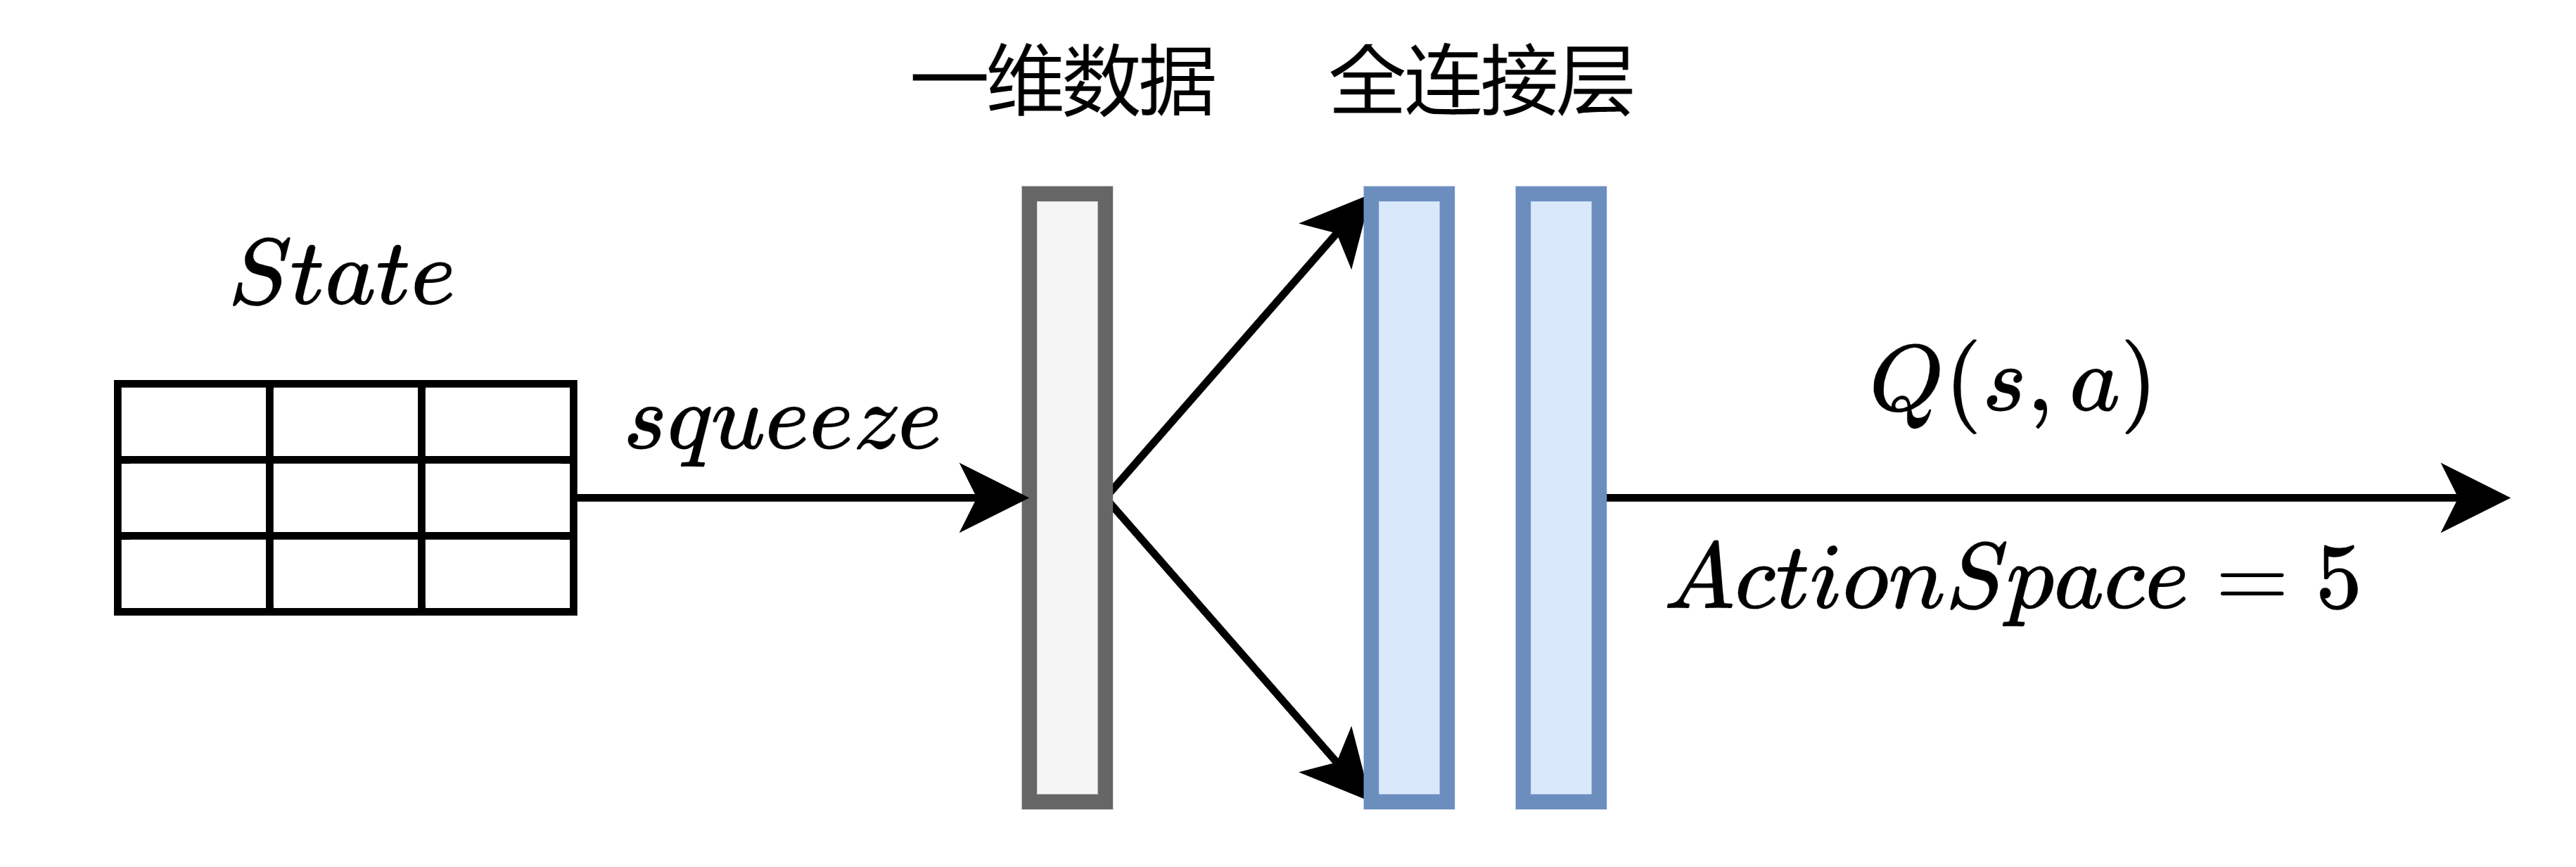
\includegraphics[width=0.73\textwidth]{images/chapter3/highway_decision.png}
    \caption{基于DQN算法的决策器网络}\label{DQN算法的决策器网络} % label 用来在文中索引
\end{figure}  

全连接层每一个结点都与上一层的所有结点相连,作用是将全连接层之前提取到的特征综合起来,最终输出行为值函数,以便后续环节的决策输出。根据前文DQN网络的相关研究,由于DQN网络需要实时的同智能体、环境交互,所以DQN网络一般采用较为简单的网络结构进行训练,其核心不在于网络结构的复杂程度,而在于算法的参数更新部分。和\ref{2.3DQN算法}节所示的DQN算法网络结构相比,Highway-Env获取的状态值是周围车辆相对于自我车辆的位置与速度,每个数据具有明确的指向性,所以不需要通过卷积层提取整体数据的特征,只采用两层的全连接层网络结构能够满足实验算法的准确度,又能保证运算速度和自动驾驶车辆决策动作的连贯。

\subsection{决策器的学习过程}

在决策器的网络结构设计结束后,决策器的算法需要根据\ref{2.3DQN算法}节所示的DQN算法进行构建。自动驾驶车辆首先获取当前的状态,每经过一个时间步,DQN算法都会对自动驾驶车辆的动作和网络结构参数进行更新。对于自动驾驶决策器而言,决策器的学习过程主要分为前向动作选取和反向数据更新两个部分。

\begin{figure}[htbp]
    \vspace{13pt}
    \centering
    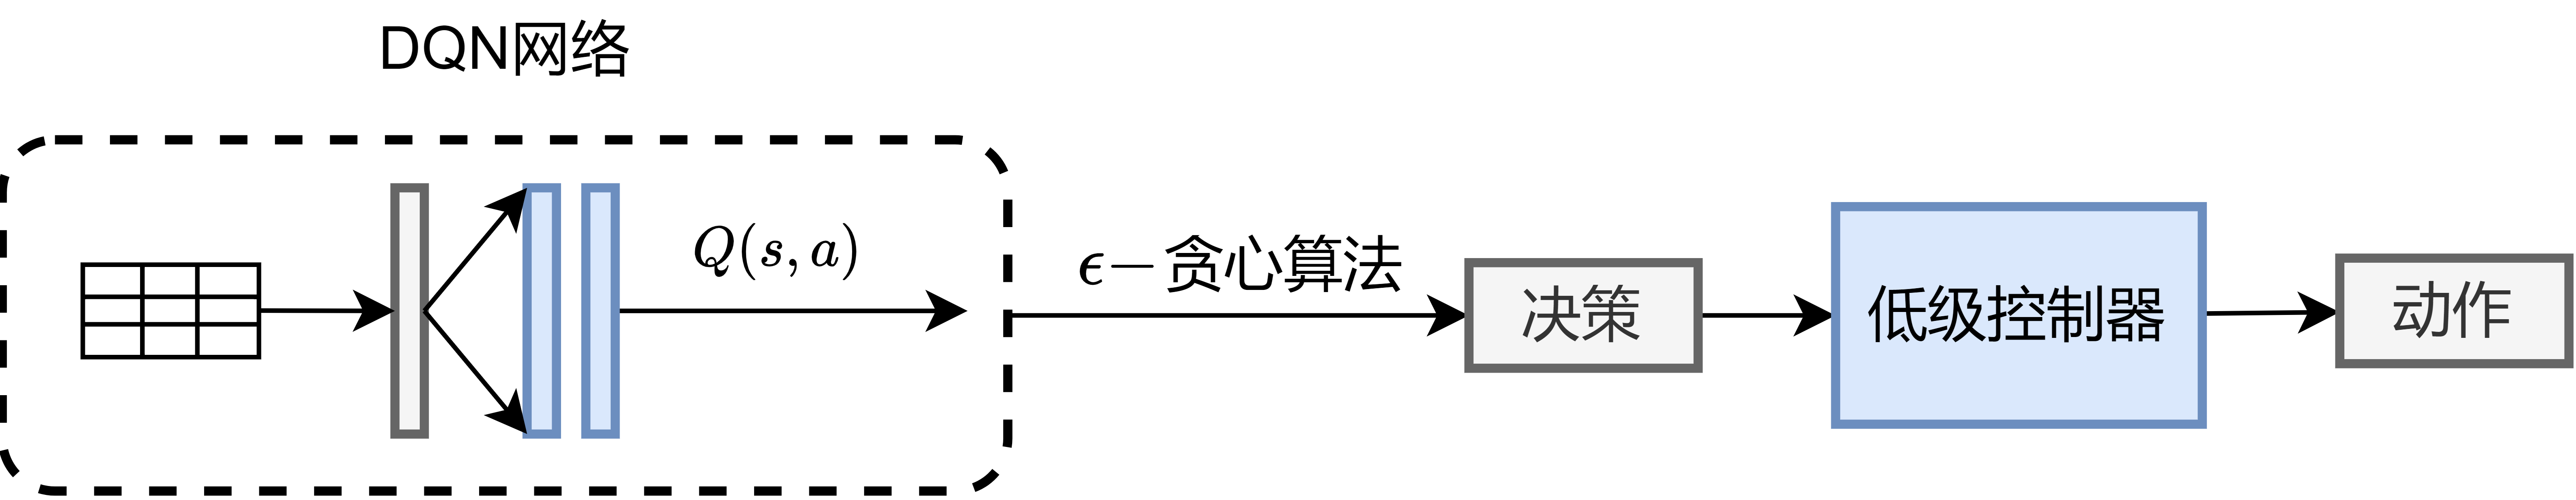
\includegraphics[width=0.85\textwidth]{images/chapter3/highway_forward.png}
    \caption{决策器前向动作选取}\label{决策器前向} % label 用来在文中索引
\end{figure}  

前向动作选取指的是在当前时刻,自动驾驶车辆将车辆当前的状态输入DQN的网络结构中,输出得到当前时刻车辆的决策动作。如图\ref{决策器前向}所示,DQN决策器网络输入自动驾驶车辆的当前状态,输出$1 \times 5$的行为值函数(Q值),在决策器学习过程中,采取$\epsilon-$贪心算法将行为值函数对应为选取的策略。每个时间步中,针对$1 \times 5$的行为值函数(Q值),以$\epsilon$概率随机选择任一随机动作,以$1-\epsilon$概率选择行为值函数最大的动作。$\epsilon$的值随着训练次数的增加而逐渐减小,在一定的训练次数后最终使得智能体选择行为值函数最大的决策动作。得到了行为值最大的决策动作,通过低级的控制器对应到Highway-Env的动作空间,从而使自动驾驶车辆完成对应的动作。

反向数据更新指的是DQN网络根据经验回放库中的数据,对DQN网络参数进行的更新。根据\ref{2.3DQN算法}节所示的DQN算法,DQN网络需要构建主网络($Q_{next}$)和TD网络($Q_{target}$),并且需要通过两者差值的平方作为损失函数进行反向传递。从经验回放库中随机采样得到数据,对每组数据的执行如下操作:

\begin{equation}
    \begin{aligned}
        q_{next} &= Q_{next}(s)\\
        q_{target} &= R(s,a) + \gamma \arg \max Q_{target}(s^{'})\\
        Loss &= MSELoss(q_{next},q_{target})\\
    \end{aligned}
\end{equation}
这里的更新方式借鉴了 Q-learning 的更新方式,最终的网络结构和参数更新通过Pytorch进行构建。

经过以上对Highway-Env仿真环境的状态值、动作值、奖励函数的说明和对DQN决策器详细的网络结构设计与分析,下一章节将以上述理论和具体实现方法作为依据,针对DQN及其改进算法在Highway-Env仿真环境中进行自动驾驶决策任务的实验验证。

\section{基于DQN算法的控制器设计} % 3.2 控制任务

\ref{3.1基于DQN算法的决策器设计}节基于DQN算法分析了自动驾驶任务决策器的设计思路,对于Highway-Env的仿真环境,输入车辆坐标等一系列抽象数据,输出运动控制的决策信息。基于端到端的方法要求直接从感知输入产生动作,当包含传感器信息输入的车辆状态维度进一步增加,直接对自动驾驶车辆的控制量(转矩与轮转角)进行离散后输出,不经过低级控制器对车辆进行实时控制,是基于DQN算法的控制器希望达成的目标。区别于Highway-Env的最小仿真环境,基于DQN算法的控制器设计需要对DQN网络的输入进行扩充,也需要更加真实的仿真环境与训练场景。

\subsection{仿真环境}

\begin{table}[htbp]
    % \vspace{13pt} % 调整图片与上文的垂直距离
    \caption{仿真模拟器对比}\label{仿真模拟器对比}
    \centering
    \renewcommand\arraystretch{1.5}
    \begin{tabular}{|c|c|c|c|c|c|}
    \hline
    Simulator   & 车辆动力学        & 多智能体       & 雷达、相机       & 真实数据导入       & 轻量级          \\ \hline
    CARLA\cite{Dosovitskiy17}       & $\checkmark$ & $\checkmark$ & $\checkmark$ & $\checkmark$ &              \\ \hline
    Metadrive\cite{li2021metadrive}   & $\checkmark$ & $\checkmark$ & $\checkmark$ & $\checkmark$ & $\checkmark$ \\ \hline
    Highway-Env\cite{highway-env} &              &              &              &              & $\checkmark$ \\ \hline
    \end{tabular}
\end{table}

MetaDrive 是一款高效的单车自动驾驶仿真模拟器\cite{li2021metadrive},和CARLA模拟器\cite{Dosovitskiy17}类似,Metadrive的状态、动作和奖励函数封装的较为完善,同时提供了较为准确的物理模型和多种传感器输入,优点是更加轻量级。多种仿真模拟器的对比如表\ref{仿真模拟器对比}所示:

Metadrive的仿真效果如图\ref{metadrive},相较于Highway-Env,它提供了更加具体的传感器输入和更加高维的观察输入,对于低级传感器(如RGB 摄像头、深度摄像头和激光雷达)可以放置在场景中的任何位置,参数可调节,同时,Metadrive还可以提供包括道路信息和附近车辆的速度和航向等高级场景信息作为状态量。本文采用Metadrive进行自动驾驶控制任务的设计。

\begin{figure}[htbp]
    \vspace{13pt} % 调整图片与上文的垂直距离
    \centering
    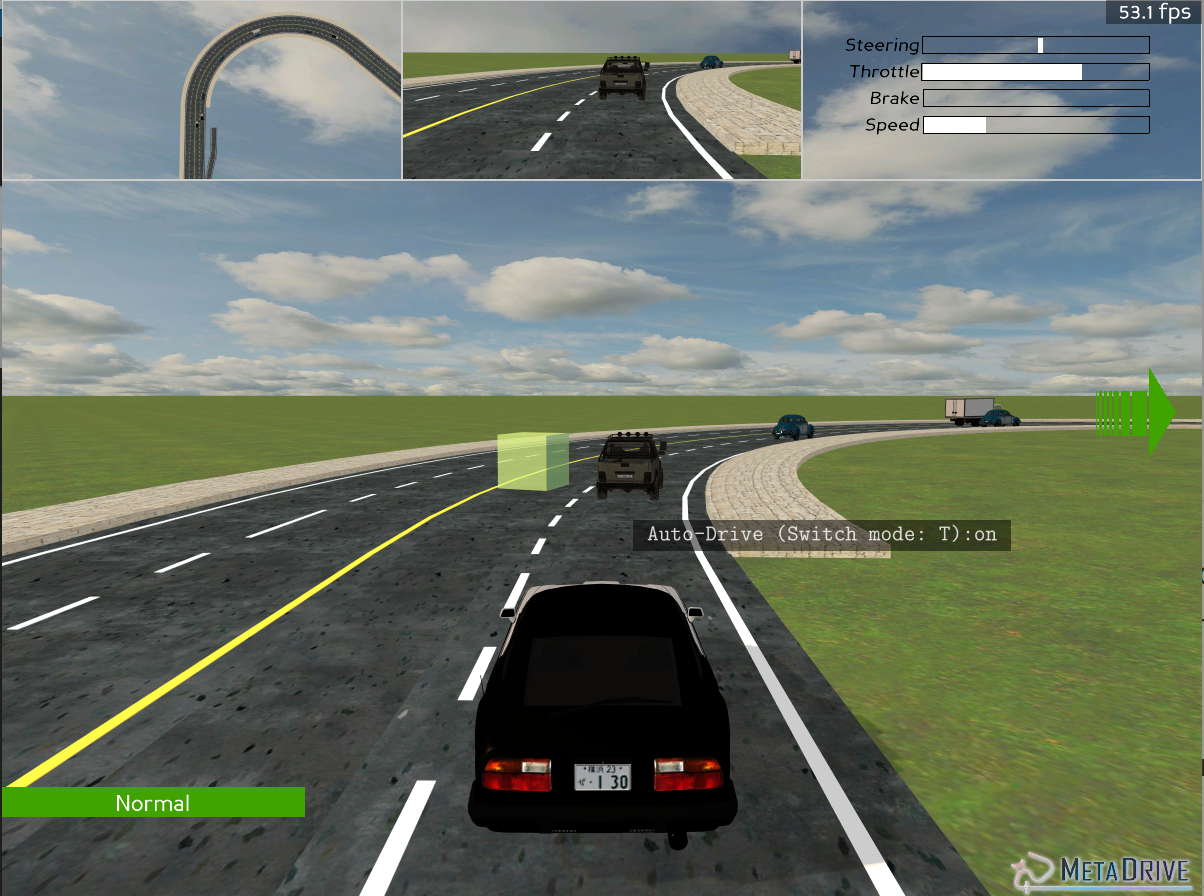
\includegraphics[width=0.73\textwidth]{images/chapter3/metadrive.png}%change
    \caption{metadrive仿真界面}\label{metadrive} % label 用来在文中索引
\end{figure}  

\subsubsection{Metadrive的状态值设计}

Metadrive提供一个状态向量,其中包含车辆导航任务所需的信息。状态向量由三部分组成:

(1) 车身状态

车身状态包括车辆当前的速度、转角、航向、控制量、横摆角速度和到边线的相对距离,这一部分包含了9个数据。

(2)导航信息

导航信息包含了引导车辆驶向目的地的信息,Metadrive首先计算车辆当前位置到目的地的路线,然后每组检查点以一定的间隔分散在整个路线上。到下一个检查点和下下一个检查点的相对距离和方向将作为导航信息给出,这一部分包含了10个数据。

(3)传感器信息

传感器信息设置为灰度相机的图像输入,周围信息通过$80\times80$的图像获取。针对于DQN算法,采用4帧$80\times80$的灰度图作为输入,这一部分包含了$4\times80\times80$个数据。

以上三部分数据在输入时都进行了归一化处理,都以$[0,1]$为区间进行了转换。

\subsubsection{Metadrive的动作值设计}

Metadrive接收标准化的动作作为输入进行车辆控制:
\begin{equation*}
    action = [steering, throttle]^{T} \in [-1,1]
\end{equation*}
在每个时间步长中,Metadrive将标准化的动作输入转换为轮转角$u_s$、发动机力$u_a$和制动力$u_b$。
\begin{equation*}
    \begin{aligned}
        u_s &= S_{max} steering\\
        u_a &= F_{max} max(0,throttle)\\
        u_b &= -B_{max} min(0,throttle)\\
    \end{aligned}
\end{equation*}
其中$S_{max}$是最大转向角,$F_{max}$是最大发动机力,$B_{max}$是最大制动力,通过这样的设计,每个智能体的动作空间总是固定的,这和标准化状态值设计是匹配的。

\subsubsection{Metadrive的奖励函数设计}

由于Metadrive所面对的环境更加复杂,故Metadrive的奖励函数也包含更多的部分,完整的奖励函数由以下三部分组成:
\begin{equation}
    R(s,a) = c_1 R_{driving} + c_2 R_{speed} + R_{termination}
\end{equation}

(1)驾驶奖励

\begin{equation*}
    \begin{aligned}
        &R_{driving} = (d_t - d_{t-1}) \times lateral\_factor\\
        &lateral\_factor = 1 - \frac{2\times lateral\_now }{lane\_width}
    \end{aligned}
\end{equation*}

其中$d_t$和$d_{t-1}$表示目标车辆在当前车道上连续两个时间步长的纵坐标,该奖励将鼓励智能体向前移动。$lateral\_factor$表示车辆是否远离了当前车道的中心,该奖励将鼓励智能体进行车道保持。

(2)速度奖励

$R_{speed} = v_t / v_{max}$,$v_t$和$v_{max}$表示当前速度与最大速度。该奖励将鼓励智能体尽可能接近$v_{max}$。

(3)终止奖励

$R_{termination}$是一组离散的奖惩函数,其包含了几种智能体可能的情况:
\begin{table}[htbp]
    \vspace{13pt}
    \centering
    \renewcommand\arraystretch{1.5}
    \begin{tabular}{|c|c|c|c|c|}
    \hline
    state & 车辆到达目的地 & 车辆驶出道路 & 车辆与其他车辆相撞 & 车辆撞到障碍物 \\ \hline
    cost  & +10.0   & -5.0   & -5.0      & -5.0    \\ \hline
    \end{tabular}
\end{table}

\subsection{网络结构设计} % 要出图,也要介绍算法的学习过程。

\begin{figure}[htbp]
    \vspace{13pt}
    \centering
    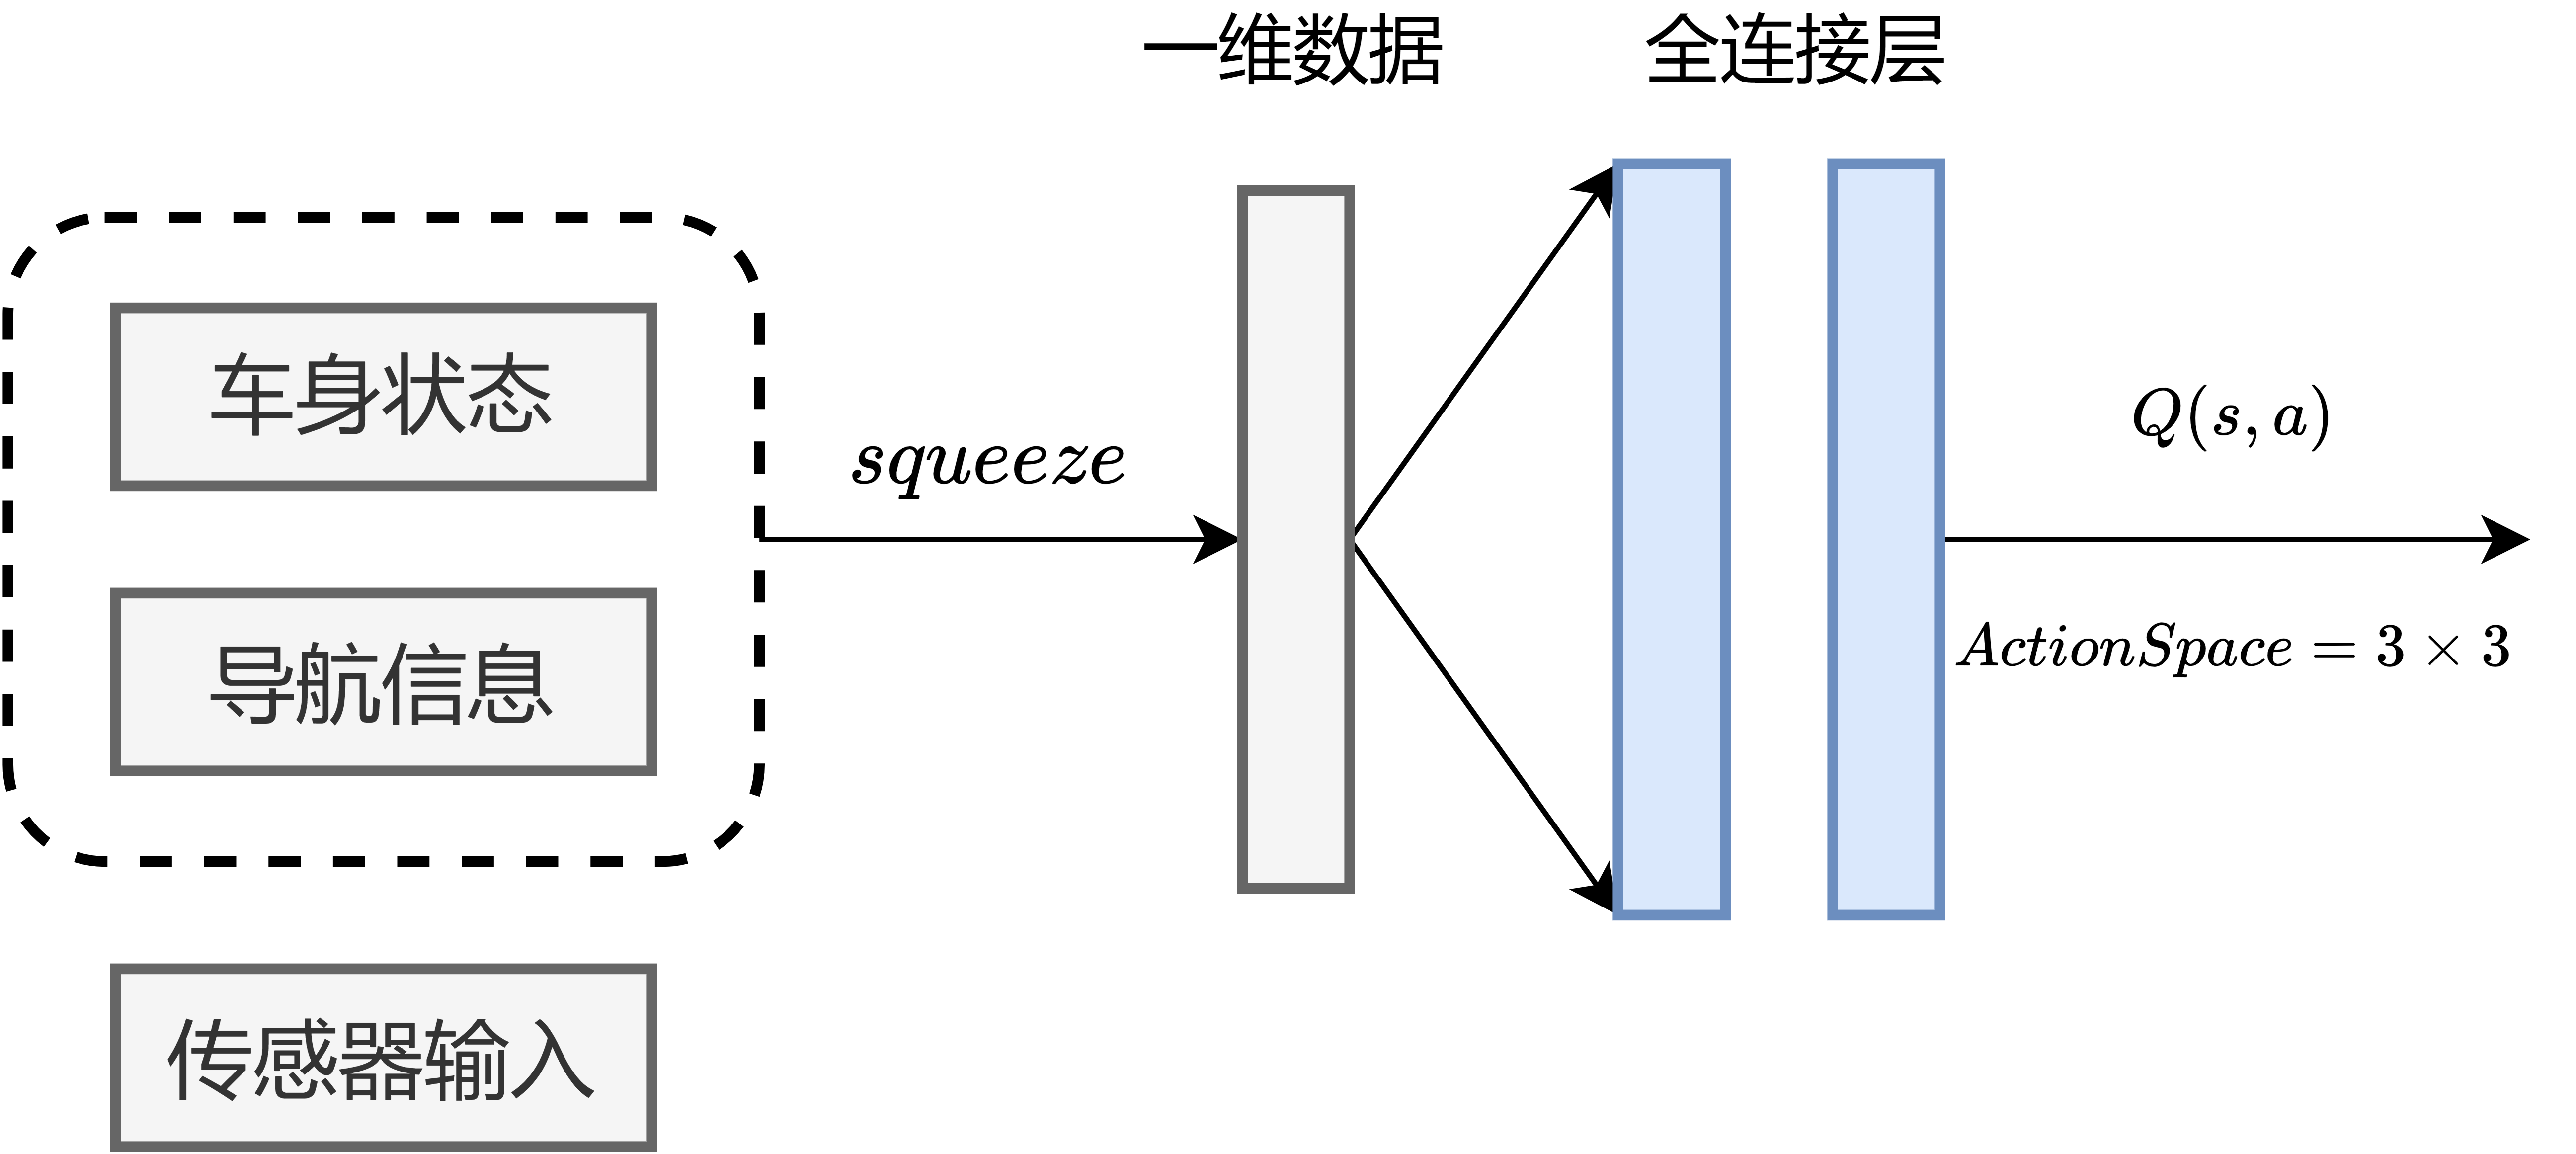
\includegraphics[width=0.73\textwidth]{images/chapter3/metadrive_control.png}
    \caption{基于DQN算法的控制器网络}\label{DQN算法的控制器网络} % label 用来在文中索引
\end{figure}  

Metadrive的状态量包括车身状态、导航信息和传感器信息,针对每个时间步长,车身状态和导航信息共包含19个数据,传感器信息包含$4\times80\times80=25600$个数据,因此前者与后者需要做出区分。网络结构设计需要明确网络结构与动作空间的大小,出于验证用途的考量,DQN的控制器设计预期实现使车辆在预定轨道上的循迹功能。参照Highway-Env的网络结构设计,仍采用两层全连接神经网络作为神经网络的结构,全连接层之间采用$relu$函数进行激活。在传感器信息方面,传感器获取周围车辆与道路信息,但是其获取的道路信息在车身状态与导航信息中已有体现,针对于车辆在预定轨道上的循迹功能,仅根据车身状态和导航信息便能依据全连接网络的综合能力完成相关任务,所以此时不将传感器信息作为网络结构的输入。具体的网络结构如图\ref{DQN算法的控制器网络}所示。

\begin{table}[htbp]
    % \vspace{13pt} % 调整图片与上文的垂直距离
    \caption{控制器动作空间}\label{控制器动作空间}
    \centering
    \renewcommand\arraystretch{1.5}
    \setlength{\tabcolsep}{7mm}{
    \begin{tabular}{|c|c|c|c|}
    \hline
    steering & -0.5 & 0 & 1   \\ \hline
    index    & 0    & 1 & 2   \\ \hline
    throttle & -0.5 & 0 & 0.5 \\ \hline
    index    & 0    & 1 & 2   \\ \hline
    \end{tabular}
    }
\end{table}

在动作空间的设计方面,动作空间分为$[steering, throttle]$两个分量,针对自动驾驶车辆的控制器而言,控制器要求在$50Hz-100Hz$的频率下做出响应,由于每个时间步长的间隔较短,且考虑到算力的限制,将连续的动作空间分为$3 \times 3$的均匀区间并对其进行编号,令$action\_index = 3 \times steering\_index + throttle\_index$,通过输出的索引确定输出的动作值。

\subsection{控制器的学习过程}

\begin{figure}[htbp]
    % \vspace{13pt}
    \centering
    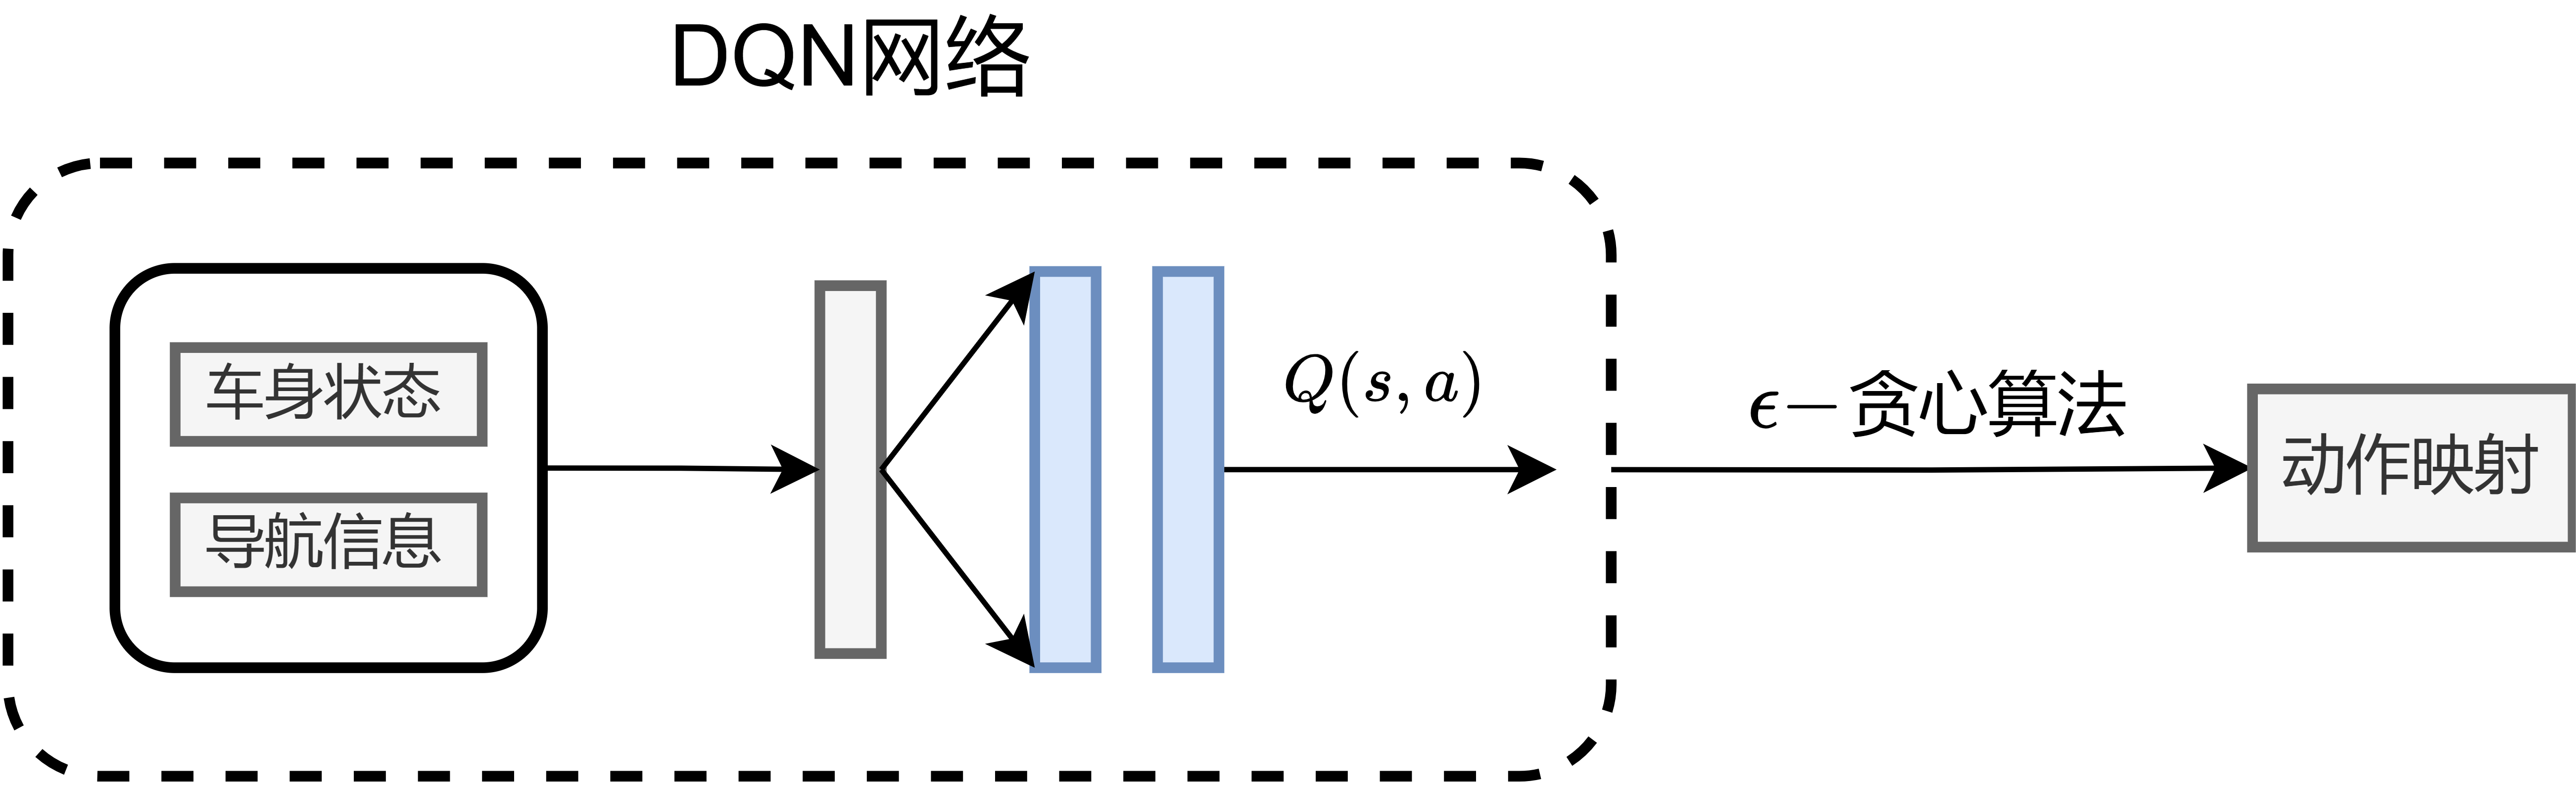
\includegraphics[width=0.85\textwidth]{images/chapter3/metadrive_forward.png}
    \caption{控制器前向动作选取}\label{控制器前向} % label 用来在文中索引
\end{figure}  

区别于Highway-Env的决策动作输出,Metadrive使用控制量进行端到端的直接输出,如图\ref{控制器前向}所示,DQN控制器网络输入自动驾驶车辆的车身状态与导航信息,输出$3 \times 3$的行为值函数(Q值),在控制器学习过程中,采取$\epsilon-$贪心算法将行为值函数对应为$action\_index$,并根据表\ref{控制器动作空间}映射到$[steering, throttle]$的实际控制量。尽管和决策器相比输入的信息含义并不相同,但通过全连接层的综合能力,能够将提取到的特征值进行综合,从而得到较为稳定的输出结果。

反向数据更新仍然是构建主网络($Q_{next}$)和TD网络($Q_{target}$),并通过两者差值的平方作为损失函数进行反向传递。从经验回放库中随机采样得到数据,对每组数据的执行如下操作:

\begin{equation}
    \begin{aligned}
        q_{next} &= Q_{next}(s)\\
        q_{target} &= R(s,a) + \gamma \arg \max Q_{target}(s^{'})\\
        Loss &= MSELoss(q_{next},q_{target})\\
    \end{aligned}
\end{equation}
这里的更新方式借鉴了 Q-learning 的更新方式,最终的网络结构和参数更新通过Pytorch进行构建。

\section{本章小结} % 3.3 本章小结

本章介绍了基于DQN及其改进型的自动驾驶避障算法设计,主要介绍了自动驾驶决策器和控制器应用的仿真环境,包括仿真环境的状态值、动作值和奖励函数的设计。在第2章算法研究的基础上,应用DQN及其改进算法,对自动驾驶决策器和控制器的网络结构设计和学习过程做了详细的分析与设计。

对于Highway-Env仿真环境,获取周围车辆相对于自我车辆的位置与速度信息,采用两层全连接神经网络拟合行为值(Q值)函数,使用DQN及其改进算法作为网络参数的更新策略,完成自动驾驶决策器的算法设计;对于Metadrive仿真环境,直接从感知输入产生动作,对自动驾驶车辆的控制量(转矩与轮转角)离散后输出,参照自动驾驶决策器的网络结构,获取车身状态与导航信息,完成车辆在预定轨道上的循迹功能。

至此,已经将基于DQN算法的决策器设计和基于DQN算法的控制器设计的理论和具体实现方法进行了详细的说明,后文将进行具体的实验对设计的算法进行验证。

 %%
% The BIThesis Template for Bachelor Graduation Thesis
%
% 北京理工大学毕业设计(论文)第四章节 —— 使用 XeLaTeX 编译
%
% Copyright 2020-2021 BITNP
%
% This work may be distributed and/or modified under the
% conditions of the LaTeX Project Public License, either version 1.3
% of this license or (at your option) any later version.
% The latest version of this license is in
%   http://www.latex-project.org/lppl.txt
% and version 1.3 or later is part of all distributions of LaTeX
% version 2005/12/01 or later.
%
% This work has the LPPL maintenance status `maintained'.
%
% The Current Maintainer of this work is Huang Chenrui.
%%

\chapter{实验验证}

\section{Highway-Env}

\section{Metadrive}


\section{改进的网络结构}

\section{结果对比}

%  \input{chapters/5_chapter5.tex}

% 结论:在结论相应的 TeX 文件处进行结论部分的撰写
%%
% The BIThesis Template for Bachelor Graduation Thesis
%
% 北京理工大学毕业设计(论文)结论 —— 使用 XeLaTeX 编译
%
% Copyright 2020-2021 BITNP
%
% This work may be distributed and/or modified under the
% conditions of the LaTeX Project Public License, either version 1.3
% of this license or (at your option) any later version.
% The latest version of this license is in
%   http://www.latex-project.org/lppl.txt
% and version 1.3 or later is part of all distributions of LaTeX
% version 2005/12/01 or later.
%
% This work has the LPPL maintenance status `maintained'.
%
% The Current Maintainer of this work is Feng Kaiyu.
%
% Compile with: xelatex -> biber -> xelatex -> xelatex

\unnumchapter{结~~~~论}
\renewcommand{\thechapter}{结论}

\ctexset{
  section/number = \arabic{section}
}

% 结论部分尽量不使用 \subsection 二级标题,只使用 \section 一级标题

% 这里插入一个参考文献,仅作参考
本文结论……。\cite{李成智2004飞行之梦}

\textcolor{blue}{结论作为毕业设计(论文)正文的最后部分单独排写,但不加章号。结论是对整个论文主要结果的总结。在结论中应明确指出本研究的创新点,对其应用前景和社会、经济价值等加以预测和评价,并指出今后进一步在本研究方向进行研究工作的展望与设想。结论部分的撰写应简明扼要,突出创新性。阅后删除此段。}

\textcolor{blue}{结论正文样式与文章正文相同:宋体、小四;行距:22 磅;间距段前段后均为 0 行。阅后删除此段。}

% 参考文献:如无特殊需要,参考文献相应的 TeX 文件无需改动,添加参考文献请使用 BibTeX 的格式
%   添加至 misc/ref.bib 中,并在正文的相应位置使用 \cite{xxx} 的格式引用参考文献
%%
% The BIThesis Template for Bachelor Graduation Thesis
%
% 北京理工大学毕业设计(论文)参考文献 —— 使用 XeLaTeX 编译
%
% Copyright 2020-2021 BITNP
%
% This work may be distributed and/or modified under the
% conditions of the LaTeX Project Public License, either version 1.3
% of this license or (at your option) any later version.
% The latest version of this license is in
%   http://www.latex-project.org/lppl.txt
% and version 1.3 or later is part of all distributions of LaTeX
% version 2005/12/01 or later.
%
% This work has the LPPL maintenance status `maintained'.
%
% The Current Maintainer of this work is Feng Kaiyu.
%
% Compile with: xelatex -> biber -> xelatex -> xelatex
%
% 如无特殊需要,本页面无需更改

% 参考文献开始
\unnumchapter{参考文献}
\renewcommand{\thechapter}{参考文献}

% 设置参考文献字号为 5 号
\renewcommand*{\bibfont}{\zihao{5}}
% 设置参考文献各个项目之间的垂直距离为 0
\setlength{\bibitemsep}{0ex}
\setlength{\bibnamesep}{0ex}
\setlength{\bibinitsep}{0ex}
% 设置单倍行距
\renewcommand{\baselinestretch}{1.2}
% 设置参考文献顺序标签 `[1]` 与文献内容 `作者. 文献标题...` 的间距
\setlength{\biblabelsep}{0.5mm}
% 设置参考文献后文缩进为 0(与 Word 模板保持一致)
\renewcommand{\itemcmd}{
  \addvspace{\bibitemsep} % 恢复 \bibitemsep 的作用
  \mkgbnumlabel{\printfield{labelnumber}}
  \hspace{\biblabelsep}}
% 删除默认的「参考文献 / Reference」标题,使用上面定义的 section 标题

% -------------------------------- 示例内容 ------------------------------------- %
% \textcolor{blue}{参考文献书写规范}

% \textcolor{blue}{参考国家标准《信息与文献参考文献著录规则》【GB/T 7714—2015】,参考文献书写规范如下:}

% \textcolor{blue}{\textbf{1. 文献类型和标识代码}}

% \textcolor{blue}{普通图书:M}\qquad\textcolor{blue}{会议录:C}\qquad\textcolor{blue}{汇编:G}\qquad\textcolor{blue}{报纸:N}

% \textcolor{blue}{期刊:J}\qquad\textcolor{blue}{学位论文:D}\qquad\textcolor{blue}{报告:R}\qquad\textcolor{blue}{标准:S}

% \textcolor{blue}{专利:P}\qquad\textcolor{blue}{数据库:DB}\qquad\textcolor{blue}{计算机程序:CP}\qquad\textcolor{blue}{电子公告:EB}

% \textcolor{blue}{档案:A}\qquad\textcolor{blue}{舆图:CM}\qquad\textcolor{blue}{数据集:DS}\qquad\textcolor{blue}{其他:Z}

% \textcolor{blue}{\textbf{2. 不同类别文献书写规范要求}}

% \textcolor{blue}{\textbf{期刊}}

% \noindent\textcolor{blue}{[序号]主要责任者. 文献题名[J]. 刊名, 出版年份, 卷号(期号): 起止页码. }

% \printbibliography [type=article,heading=none] 

% \textcolor{blue}{\textbf{普通图书}}

% \noindent\textcolor{blue}{[序号]主要责任者. 文献题名[M]. 出版地: 出版者, 出版年. 起止页码. }
% \cite{Raymer1992Aircraft}

% \printbibliography [keyword={book},heading=none] 

% \textcolor{blue}{\textbf{会议论文集}}

% \noindent\textcolor{blue}{[序号]析出责任者. 析出题名[A]. 见(英文用In): 主编. 论文集名[C]. (供选择项: 会议名, 会址, 开会年)出版地: 出版者, 出版年. 起止页码. }
% \cite{sunpinyi}

% \printbibliography [type=inproceedings,heading=none] 

% \textcolor{blue}{\textbf{专著中析出的文献}}

% \noindent\textcolor{blue}{[序号]析出责任者. 析出题名[A]. 见(英文用In): 专著责任者. 书名[M]. 出版地: 出版者, 出版年.起止页码. }
% \cite{luoyun}

% \printbibliography [type=inbook,heading=none] 

% \textcolor{blue}{\textbf{学位论文}}

% \noindent\textcolor{blue}{[序号]主要责任者. 文献题名[D]. 保存地: 保存单位, 年份. }
% \cite{zhanghesheng}
% \cite{Sobieski}

% \printbibliography [keyword={thesis},heading=none] 

% \textcolor{blue}{\textbf{报告}}

% \noindent\textcolor{blue}{[序号]主要责任者. 文献题名[R]. 报告地: 报告会主办单位, 年份. }
% \cite{fengxiqiao}
% \cite{Sobieszczanski}

% \printbibliography [keyword={techreport},heading=none] 

% \textcolor{blue}{\textbf{专利文献}}

% \noindent\textcolor{blue}{[序号]专利所有者. 专利题名[P]. 专利国别: 专利号, 发布日期. }
% \cite{jiangxizhou}

% \printbibliography [type=patent,heading=none] 

% \textcolor{blue}{\textbf{国际、国家标准}}

% \noindent\textcolor{blue}{[序号]标准代号. 标准名称[S]. 出版地: 出版者, 出版年. }
% \cite{GB/T16159—1996}

% \printbibliography [keyword={standard},heading=none] 

% \textcolor{blue}{\textbf{报纸文章}}

% \noindent\textcolor{blue}{[序号]主要责任者. 文献题名[N]. 报纸名, 出版年, 月(日): 版次. }
% \cite{xiexide}

% \printbibliography [keyword={newspaper},heading=none] 

% \textcolor{blue}{\textbf{电子文献}}

% \noindent\textcolor{blue}{[序号]主要责任者. 电子文献题名[文献类型/载体类型]. 电子文献的出版或可获得地址(电子文献地址用文字表述), 发表或更新日期/引用日期(任选). }
% \cite{yaoboyuan}

% \printbibliography [keyword={online},heading=none] 

% \textcolor{blue}{关于参考文献的未尽事项可参考国家标准《信息与文献参考文献著录规则》(GB/T 7714—2015)}

% 在使用时,请删除/注释上方示例内容,并启用下方语句以输出所有的参考文献
\printbibliography[heading=none]

% 附录:在附录相应的 TeX 文件处进行附录部分的撰写
% %%
% The BIThesis Template for Bachelor Graduation Thesis
%
% 北京理工大学毕业设计(论文)附录 —— 使用 XeLaTeX 编译
%
% Copyright 2020-2021 BITNP
%
% This work may be distributed and/or modified under the
% conditions of the LaTeX Project Public License, either version 1.3
% of this license or (at your option) any later version.
% The latest version of this license is in
%   http://www.latex-project.org/lppl.txt
% and version 1.3 or later is part of all distributions of LaTeX
% version 2005/12/01 or later.
%
% This work has the LPPL maintenance status `maintained'.
%
% The Current Maintainer of this work is Feng Kaiyu.
%
% Compile with: xelatex -> biber -> xelatex -> xelatex

\unnumchapter{附~~~~录}
\renewcommand{\thechapter}{附录}

% 设置附录编号格式
\ctexset{
  section/number = 附录\Alph{section}
}

附录相关内容…

% 这里示范一下添加多个附录的方法:

\section{\LaTeX 环境的安装}
\LaTeX 环境的安装。

\section{BIThesis 使用说明}
BIThesis 使用说明。


% 致谢:在致谢相应的 TeX 文件处进行致谢部分的撰写
% %%
% The BIThesis Template for Bachelor Graduation Thesis
%
% 北京理工大学毕业设计(论文)致谢 —— 使用 XeLaTeX 编译
%
% Copyright 2020-2021 BITNP
%
% This work may be distributed and/or modified under the
% conditions of the LaTeX Project Public License, either version 1.3
% of this license or (at your option) any later version.
% The latest version of this license is in
%   http://www.latex-project.org/lppl.txt
% and version 1.3 or later is part of all distributions of LaTeX
% version 2005/12/01 or later.
%
% This work has the LPPL maintenance status `maintained'.
%
% The Current Maintainer of this work is Feng Kaiyu.
%
% Compile with: xelatex -> biber -> xelatex -> xelatex

\unnumchapter{致~~~~谢}
\renewcommand{\thechapter}{致谢}

\ctexset{
  section/number = \arabic{section}
}

% 致谢部分尽量不使用 \subsection 二级标题,只使用 \section 一级标题

修修改改缝缝补补,从2022年5月2号创建的第一版Github-repo开始,历时近一个月,总算根据多方意见完成了论文写作。值此论文完成之际,我想向我的导师宋春雷表示诚挚的敬意和衷心的感谢。从论文选题伊始,老师委托丁子豪学长对我悉心的指导和建议,我也开始对论文写作和深度强化学习有了初步的了解和认识。是老师和学长的殷切教导,才使得盲审有了一个好的结果。

其次,我想感谢一路陪伴我的父母、家人,家人永远是我的坚强后盾,没有你们的帮助和支持,我不可能顺利的完成学业。纵使出现了一些变故,但你们的支持使我接续奋斗。

在大学四年的科创活动中,我特别感谢的是北京理工大学无人驾驶方程式赛车队(Beijing Institute of Technology
Driverless Racing Team, BITFSD)。感谢陈泰然学长、马宁博士、高欣彧、杨少坤、龚海龙、吕文成、封蕴籍、李云巍……没有车队这样的专注于科研和实践相结合的团队,我不会对自动驾驶产生这样的兴趣,也不会随队捧杯。

特别关键的,我想感谢北京理工大学交响乐团合唱团艺术总监贺春华教授,感谢音乐的力量。在大学四年的学习生活中,虽然我作为仅仅来唱唱歌的同学,也许只是过客,但我仍然获得了合唱艺术、声乐艺术美的感受。同时感谢合唱团的朋友们,李瀚宇、葛易谙、张柏灵、袁海洋、杨峰、王首智……“他们应该是”一群热爱音乐的朋友们,来日方长,后会有期(呵呵)。

大学四年,即将毕业,即将工作。感谢上汽通用泛亚汽车技术中心有限公司的Offer、感谢金龙联合汽车工业(苏州)有限公司提供的实习机会。

请你别忘了我,Non ti scordar di me。

\end{document}
